\cleardoublepage
\chapter{Safely learning with kernels}
\markboth{Learning with kernels}{Learning with kernels}

\section{Introduction}
At its core, learning refers to the process of gathering information and using it to improve one's knowledge about the phenomenon under study, which we will call the ground-truth. The standing assumption is that a link is in place, tying information and the ground-truth together even if such link is partially corrupted. Information typically comes in the form of data, samples, sometimes referred to as examples, and
%In modern machine learning, people study a number of rather abstract subjects ranging from the traits that distinguish images of muffins and chihuahuas, to the link between passengers' features and their survival likelihood in case of a ship sinking event.  
the mathematical formalism often used in modern machine learning to study the link between examples and the underlying phenomena is statistics. This choice is convenient because it can describe the possible non-determinism of outcomes through the concepts of distributions and samples; and because it provides us with plenty of tools to carry out learning, i.e., improve our knowledge about the phenomenon through the samples at hand. In this chapter, we will however adopt a different standpoint to study the problem of learning, relying on an \textit{epistemic} description of uncertainty rather than on an aleatoric one \citep{hullermeier2021aleatoric}.

When reporting physical parameters that are not exactly known, e.g. the friction coefficient between two surfaces or the leakage inductance of a transformer, it is common for engineers to specify ranges that are known to contain the \textit{true} coefficient values. Assuming that a true, invariable value exists although it is not exactly known is the epistemic way of modeling uncertainty. This approach is customary in many applied sciences and can be generalized from simple scalar parameters to maps in function spaces. The entire field of approximation theory, from which we will borrow many tools, makes constant use of this framework to derive best approximations and error bounds for their nominal models \citep{wendland2004scattered,iske2018approximation}.  Let us refer to this space as the ground-truth space (GTS), whereas the space from where our models are drawn will be called the hypothesis space (HS). An advantage of working with functions spaces is the ease of packing information into them that we might have as domain experts: take for instance the Lipschitz continuity explored in  \cite{milanese2004set,sabug2021smgo} or the weak derivatives assumptions in Sobolev GTSs by the authors of \cite{novara2022nonlinear}. In this chapter, rather than posing assumptions directly on the ground-truth, we will make use of an indirect formalism that ties the GTS to maps named \textit{kernels}. This approach guarantees the existence of a rich geometrical structure that will allow us to develop our theory.

Kernels are a fundamental building block of modern machine learning \citep{scholkopf2002learning}. They enable computing similarities in extended feature spaces while dispensing with the need of lifting the data onto them. Alternatively, they can be viewed as a non-linearity library used to empower certain linear algorithms, the canonical example being support vector machines. If kernels are used to describe simultaneously the HS and the GTS, then not only optimal models can be found, but also error-bounds can be derived for them at possibly out-of sample locations, thus guaranteeing the quality of the model predictions \citep{schaback2006kernel,kanagawa2018gaussian}. One interesting aspect of those bounds are their determinism, in that the ground-truth values cannot lie outside the established ‘prediction envelope’. Therefore, such methods could in principle be used in the engineering sciences to deterministically certify the performance or safety of algorithms that employ learned maps, which is remarkable due to their not being asymptotic, but finite-sample guarantees. There is however one strong limiting factor that hinders its applicability, namely the absence of a noise model \citep[§11]{wendland2004scattered}. Even though noise-free samples are to be expected in domains such as computer graphics and  computer simulations, where these techniques are usually applied  (see e.g. \citep{sarra2005adaptive,nikan2022numerical}), corrupted data is prevalent in electronics, robotics, building automation, among other fields. 

In this chapter, we will explore kernel learning with hard guarantees. Our contributions, which are mainly reported in Section~\ref{sec.quant_uncert}, consist in posing and solving an uncertainty quantification (UQ) problem to compute envelopes that bound the unknown ground-truth values. We highlight that the UQ problem does not require defining a nominal model, being thus agnostic to its choice. As opposed to other deterministic bounds found in the literature (see the classical book \citep[§11]{wendland2004scattered}), ours take encompass an additive noise with bounded levels, a description that is not popular in general machine learning, but certainly relevant in domains such as robust analysis and control. A number of examples are presented at the end to illustrate different use-cases for the proposed theory, followed by concluding remarks and ideas for future investigations.

%\footnote{Approximation theory is not in complete opposition to statistical learning. Indeed, we can define the function of interest as the conditional \citep{temlyakov2008approximation}.}
% See also the work of \cite{belkin2018approximation} comparing the two views.}
%In this chapter, we will introduce the problem of learning from data and elucidate what approach will be taken to tackle it. Next, novel uncertainty quantification results will be presented concerning the point-evaluations of an  unknown ground-truth. Finally, some examples are given to illustrate the general use of the theory.

\section{The formalism of kernels}
\label{sec.formalism_of_kernels}

Our goal in to learn maps of the form $f: \mathcal{X} \rightarrow \mathbb{R}$ and, to achieve that end, we will make extensive use of auxiliary functions called kernels.

\begin{definition}
	\textbf{(Kernel)} Given an arbitrary non-empty set $\mathcal{X}$, a kernel $k$ is any symmetric function of the form
	\begin{equation}
		k: \mathcal{X} \times \mathcal{X} \rightarrow \mathbb{R}
	\end{equation}
\end{definition}

\begin{definition}
	\textbf{(Kernel matrix)} Let $X = \{x_1,\dots,x_n\} \subset \mathcal{X}$ be a finite set of points. The $n \times n$ matrix $K_{XX}$ with entries $[K_{XX}]_{ij} = k(x_i,x_j)$ is called the kernel matrix of $k$ associated with $X$.
\end{definition}

\begin{definition}
	\label{def.pd_kernel}
	\textbf{(Positive-definite kernel)} A kernel function $k$ is said to be positive-definite if for any finite subset of points $X \subset \mathcal{X}$, the kernel matrix satisfies $K_{XX} \succeq 0$. If, in particular, $K_{XX} \succ 0$, then the kernel is strictly positive-definite.
\end{definition}

\begin{remark}
	Aside from the last definition, there exist broader classes of kernel functions such as the \textit{conditionally positive-definite} one \cite[§2.4]{scholkopf2002learning}\cite[§8]{wendland2004scattered}. In addition, one can also generalize the co-domain $k$ to be the field of complex numbers $\mathbb{C}$.
\end{remark}

Instances of positive-definite kernel functions with index set $\mathcal{X} = \mathbb{R}^n$ are the linear, the squared-exponential (also known as Gaussian), the exponential (equivalent to the Matern12), the polynominal and the cosine kernels respectively given by
\begin{align}
	&k_\text{lin}(x,x') = x \cdot x' \\
	&k_\text{se}(x,x') = \exp\left(-\frac{\Vert x-x'\Vert^2}{2\ell}\right) \label{eq.se_kernel}\\
	&k_\text{exp}(x,x') = \exp\left(-\frac{\Vert x-x'\Vert}{2\ell}\right) \\
	&k_\text{pol}(x,x') = \left(\sigma^2 (x \cdot x') + \gamma \right)^d \\
	&k_\text{cos}(x,x') = \cos\left(2\pi \sum_i ([x]_i-[x']_i)/\ell \right)
\end{align}
where $\cdot$ and $\Vert \cdot \Vert$ denote the usual inner-product  and 2-norm in $\mathbb{R}^n$, respectively; and the constants $\ell \in \mathbb{R}_{>0}$, $\sigma, \gamma\in \mathbb{R}$ are the so-called \textit{hyperparameters}. Plots of these functions are presented in Figure~\ref{fig.pd_kernels}. A more complete list of PD kernels and their mathematical properties can be found in Appendix~A. 

In order to construct surrogate models for the unknown $f$, one could partially evaluate a given $k$ to match their domains and co-domains. In other words, fix one of its arguments so that $k(z,\cdot): \mathcal{X} \rightarrow \mathbb{R}, x \mapsto k(z,x)$ for some $z \in \mathcal{X}$. Indeed, this was the approach taken to draw the plots in Figure~\ref{fig.pd_kernels}. Approximating the unknown $f$ with a single partially evaluated kernel however appears to be overly restrictive. A sensible next step would be to consider linear combinations of such kernel functions. It turns out that every PD kernel has a function space associated with it that contains these linear combinations and is endowed with plenty of useful geometric structure. The following concepts are presented next to set up the stage for defining this special hypothesis space, the \textit{reproducing kernel Hilbert space}.

\begin{figure}[t]
	\centering
	\includegraphics{../images/chap2_kernel_li.pdf} \hspace{3pt}
	\includegraphics{../images/chap2_kernel_se.pdf} \hspace{3pt}
	\includegraphics{../images/chap2_kernel_ex.pdf} \\[3pt]
	\includegraphics{../images/chap2_kernel_pl.pdf} \hspace{3pt}
	\includegraphics{../images/chap2_kernel_cs.pdf} \hspace{3pt}
	\includegraphics{../images/chap2_kernel_csli.pdf} 
	\caption{Examples of positive-definite kernels.}
	\label{fig.pd_kernels}
\end{figure}


Feature maps $\Phi$ are central in machine learning, allowing one to represent the data $x$ he has in a more suitable format. At the same time, \eqref{eq.kernels_feat_maps} unveils another aspect of a kernel evaluation $k(x,x')$: it returns the inner-product value of the transformed inputs $\Phi(x)$, $\Phi(x')$. Educational textbooks often interpret these inner-products as a similarity measure between $x$ and $x'$ \citep{scholkopf2002learning}.

\begin{proposition}
	\label{thm.pd_kernels_feature_maps}
	\textbf{(PD kernels have feature maps)} 
	Let $k:\mathcal{X} \times \mathcal{X} \rightarrow \mathbb{R} $ be a positive-definite kernel. Then there exists a Hilbert space $\mathbb{H}$ endowed with an inner product $\langle \cdot,\cdot \rangle_\mathbb{H}$ and a mapping $\Phi :  \mathcal{X} \rightarrow \mathbb{H}$ such that 
	\begin{equation}
		\label{eq.kernels_feat_maps}
		k(x,x') = \langle \Phi(x),\Phi(x') \rangle_\mathbb{H}
	\end{equation}
	holds for any $x,x' \in \mathcal{X}$.
\end{proposition}

\begin{my_proof}
	\textbf{Proof.}
	\cite[Theorem~4.16]{steinwart2008svm_book}, modulo the nomenclature difference.
\end{my_proof}

The mappings $\Phi$ above as well as the $\mathbb{H}$ spaces are in general not unique \citep[§4]{steinwart2008svm_book}, but there is one such space that enjoys an extra property that rules out some unexpected behavior from its members. This particular $\mathbb{H}$ is moreover not an arbitrary Hilbert space, but a Hilbert space of functions.

\begin{definition}
	\label{def.rkhs}
	\textbf{(Reproducing kernel Hilbert space)} 
	Let $\mathcal{X} \neq \emptyset$ and $\mathbb{R}^\mathcal{X}$ the set of functions mapping $\mathcal{X}$ to $\mathbb{R}$. The subset $\mathcal{H} \subset \mathbb{R}^\mathcal{X}$ is called a reproducing kernel Hilbert space (RKHS) if it is a Hilbert space and if $\forall x \in \mathcal{X}$ the evaluation functionals
	\begin{equation}
		L_x: \mathcal{H} \rightarrow \mathbb{R}, \; L_x(f) \mapsto f(x), \ \forall f\in \mathcal{H}
	\end{equation}
	are bounded.
\end{definition}

In order to see how useful such a property is, consider a sequence $\{f_n\}_{n=1}^\infty$ within a certain Hilbert function space $\mathbb{H} \subset \mathbb{R}^\mathcal{X}$. Intuitively, one would expect that if $f_n \rightarrow f^\star$ in $\mathbb{H}$, then the values $f_n(x)$ attained by the sequence would converge to the values $f^\star(x)$. Yet, this is not always the case (see Example~\ref{ex.appendix_convergence} in Appendix~\ref{app.elements_analysis_algebra}). If, on the other hand, the evaluation functionals are bounded as in Definition~\ref{def.rkhs}, then the connection between convergence in the function space and the pointwise convergence of functions is guaranteed. Indeed, if $\{f_n\}_{n=1}^\infty$ and $f^\star$ are members of an RKHS $\mathcal{H}$, then $|f_n(x)-f^\star(x)| = | L_x(f_n) - L_x(f^\star)|  \leq \Vert L_x \Vert \rknorm{f_n - f^\star}$, where $\Vert L_x \Vert $ is the operator norm of $L_x$ that is guaranteed by Definiton~\ref{def.rkhs} to be a finite number. As a result, if $\rknorm{f_n - f^\star} \rightarrow 0$, the right-hand side of the inequality goes to zero, and so does the pointwise difference $|f_n(x)-f^\star(x)|$. Therefore, function convergence in an RKHS implies pointwise convergence, matching our intuition.

\begin{proposition}
	\label{prop.unique_reprod_kernel}
	\textbf{(Every RKHS has a unique PD reproducing kernel)} 
	Let $\mathcal{H} \subset \mathbb{R}^\mathcal{X}$ be an RKHS. Then, the map $k: \mathcal{X} \times \mathcal{X} \rightarrow \mathbb{R}$, $k(x,x') := \langle L_x, L_{x'} \rangle_\mathcal{H}$ is a positive-definite kernel. Furthermore, $k$ is the unique map to satisfy the reproducing property, i.e., for any $x \in \mathcal{X}$, $k(x,\cdot) \in \rkhs$ and
	\begin{equation}
		\rkinner{f}{k(x,\cdot)} = L_x(f) = f(x), \ \forall f \in \rkhs
		\label{eq.reproducing_property}
	\end{equation} 
\end{proposition}

\begin{my_proof}
	\textbf{Proof.}
	 \cite[Lemma~2]{berlinet2011reproducing} along with \citep[Theorem~4.20]{steinwart2008svm_book}.
\end{my_proof}

\begin{proposition}
	\label{prop.unique_rkhs}
	\textbf{(Every PD kernel has a unique RKHS)} 
	Let $k: \mathcal{X} \times \mathcal{X} \rightarrow \mathbb{R}$ be a PD kernel. If $k$ is the reproducing kernel of an RKHS $\rkhs_A$ and of another RKHS $\rkhs_B$, then $\rkhs_A = \rkhs_B$.
\end{proposition}

\begin{my_proof}
	\textbf{Proof.}
	\citep[Theorem~4.21]{steinwart2008svm_book}.
\end{my_proof}

We understand from Propositions~\ref{prop.unique_reprod_kernel} and \ref{prop.unique_rkhs} that a special relationship exists between kernel and its RKHS. Nevertheless, it is still unclear from Definition~\ref{def.rkhs} alone how a given $k$ influences or defines the members of $\rkhs$. To shed light on the matter, it helps to explicitly construct $\rkhs$ starting from a given $k$. Consider the so-called \textit{pre-Hilbert space}
\begin{empheq}[box={\mymathbox[colback=black!2,drop small lifted shadow, sharp corners]}]{align}
	\rkhs_0 :=& \; \text{span} \, \{ k(x,\cdot) \, | \, x \in \mathcal{X} \} \\
 	=&  \; \left\{ \sum_{i=1}^n c_i \, k(x_i,\cdot) \, | \, n \in \mathbb{N}, c_i \in \mathbb{R}, x_i \in \mathcal{X} \right\} \label{eq.pre_rkhs}
\end{empheq}
equipped with the real-valued map $\langle f,g\rangle_{\mathcal{H}_0} := \sum_{i=1}^n \sum_{j=1}^m a_i b_i k(x_i,x_j)$ for members $f,g \in \mathcal{H}_0, f=\sum_{i=1}^n a_i \, k(x_i,\cdot), g=\sum_{j=1}^m b_j \, k(x_j,\cdot) $, which can be shown to be a valid inner-product. This family $\mathcal{H}_0$ of functions is however not guaranteed to be complete, i.e., sequences $\{f_i\}_{i\in\mathbb{N}}$ of members might converge to functions outside $\mathcal{H}_0$. To transform it into a proper Hilbert space, one closes the space 
\begin{empheq}[box={\mymathbox[colback=black!2,drop small lifted shadow, sharp corners]}]{equation}
	\label{eq.rkhs_closure}
	\mathcal{H} := \text{clos} \, \mathcal{H}_0
\end{empheq}
%\begin{equation}
%	\mathcal{H} := \text{clos} \, \mathcal{H}_0
%\end{equation}
thus encompassing all limit points\footnote{
%
Closing $\mathcal{H}_0$ requires defining an inner-product on the superset $\rkhs$ that is consistent with the one present in the subset $\mathcal{H}_0$. Also, the closure of a set is always closed, which guarantees that sequences within $\mathcal{H}$ cannot converge to functions outside of it.
%
}. Finally, the function space $\mathcal{H}$ defined in \eqref{eq.rkhs_closure} can then be shown to be a valid RKHS\footnote{
%
For a proof of this statement, the reader is referred to \cite[§3]{berlinet2011reproducing} or to \cite[§4]{sejdinovic2012rkhs} for a more step-by-step pedagogical exposition.
%
} according to Definition~\ref{def.rkhs}. In fact, it is the \textit{only} one associated with $k$. We therefore understand that the members of $\rkhs$ are weighted sums of partially evaluated kernels as per \eqref{eq.pre_rkhs} along with their limit points. 
%and requires showing that the elements included through the closure are indeed functions with well-defined point evaluations \cite[§4]{aronszajn1950theory}\cite[§10.2]{wendland2004scattered}, a step that is overlooked in simplified presentations.

The questions of how expressive RKHSs can be still lingers on. To better examine the matter, consider the following measure of expressiveness.

\begin{definition}
	\textbf{(Universal kernel)}
	\label{def.universal_kernel}
	Let $k$ be a continuous PD kernel and the set $\mathcal{X}$ be a compact metric space. Then $k$ is called universal if its RKHS $\rkhs \subset \mathbb{R}^\mathcal{X}$ is dense in the space of real-valued continuous functions $C(\mathcal{X}) \subset \mathbb{R}^\mathcal{X}$ with respect to the maximum norm $\Vert \cdot \Vert_\infty$.
\end{definition}

The above definition guarantees that for any target function $g \in C(\mathcal{X})$ and any tolerable error $\epsilon > 0$, there exists an $f$ in the RKHS of a universal kernel such that their mismatch is bounded $| f(x) - g(x) | \leq \epsilon, \forall x \in \mathcal{X}$.
% REFINE
All in all, the universality property is an indication of how rich a hypothesis space is, thus reassuring the user that little bias error will be introduced by his choice of model class.

\begin{proposition}
	\label{prop.univ_kernels}
	Let $\mathcal{X}$ be a compact subset of $\mathbb{R}^n$. The squared-exponential kernel with \eqref{eq.se_kernel} with $\ell >0$ is universal.
\end{proposition}

\begin{my_proof}
	\textbf{Proof.}
	\cite[Corollary~4.58]{steinwart2008svm_book}.
\end{my_proof}

In contrast with Proposition~\ref{prop.univ_kernels}, some results on the restrictiveness of RKHSs can also be found in the literature. In \cite{steinwart2020_no_rkhs_cont_func} for example, the author shows that no RKHS can contain $C(X)$. On a looser note, some authors argue that members of the squared-exponential kernel \eqref{eq.squared_exponential} has an $\rkhs$ that is too smooth when compared to alternative hypothesis spaces that are also associated with the same kernel (see the discussion in \cite[§4]{kanagawa2018gaussian}). For a thorough exposition of universal kernels, the reader is referred to \cite{micchelli2006universal}. Lastly, we underline that other model classes in machine learning also enjoy the same universality properties that kernels do, notable certain architectures of deep neural networks \citep{kidger2020universal}.

\begin{landscape}
\begin{figure}
	\includegraphics{../images/chap2_rkhs_ex.pdf} 
	\caption{Members of the exponential RKHS and their respective norms.}
	\label{fig.rkhs_ex}
\end{figure}
\end{landscape}


\section{Crafting models}
\label{sec.crafting_models}

Suppose a dataset of the form $\{(x_i,y_i)\}_{i=1}^n$ is given. The $x_i \in \mathcal{X}, \forall i$ elements are referred to as \textit{inputs} and the $y_i \in \mathbb{R}, \forall i$ as \textit{outputs}. In this section, we will discuss exclusively the case where $\mathcal{X} \subset \mathbb{R}^m$ is a compact set, and the outputs are real-valued. The values $y_i$ are assumed to deliver information about an underlying ground-truth function $f^\star$ through the measurement model
\begin{equation}
	y_i = f^\star(x_i) + \epsilon_i, \quad i=1,\dots,n
\end{equation}

As detailed in Section~\ref{sec.formalism_of_kernels}, weighted sums of partially evaluated kernel functions arise naturally in the context of kernel learning. In this section we shall see that, when given $\{(x_i,y_i)\}_{i=1}^n$, maps of the form
\begin{equation}
	f(x) = \sum_{i=1}^n \alpha_i k(x_i,x)
\end{equation}
are good candidates for acting as surrogate functions for the ground-truth $f^\star$. Indeed, they are known to solve a number of optimal fitting problems given appropriate weights $\alpha$ as we explain next.

In the absence of measurement noise, i.e., when $\epsilon_i = 0$, the outputs $y_i$ perfectly represent $f^\star$. As a result, data interpolation can be a sensible task to carry out, which could done over $f \in \rkhs$ while minimizing the resulting model norm.
%\begin{align}
%		\bar{f} = \arginf_{f \in \mathcal{H}} & \quad \rknorm{f}^2 \\
%		\text{subj. to} & \quad f(x_i) = y_i, \, i = 1,\dots,n 
%\end{align}
\begin{proposition}
	\label{prop.MNI}
	\textbf{(Minimum-norm interpolation (MNI))}
	Let $\{(x_i,y_i)\}_{i=1}^n$ be a collection of points such that $x_i \in \mathbb{R}^m$ and $y_i \in \mathbb{R}$. Let $k$ be a PD kernel and $\rkhs \subset \mathbb{R}^\mathcal{X}$ its RKHS. Then, the variational problem
	\begin{equation}
		\label{eq.min_norm_interp}
			\bar{f} \in \arginf_{f \in \mathcal{H}} \left\{ \rknorm{f}^2 : f(x_i) = y_i, \, i = 1,\dots,n \right\}
	\end{equation}
	admits the unique solution $\bar f \in \rkhs$, $\bar f(x) =  \sum_{i=1}^n \alpha_i k(x_i,x)$, $\alpha = y^\top K_{XX}^{-1}$.
\end{proposition}
\begin{my_proof}
	\textbf{Proof.}
	\cite[Theorem~3.5]{kanagawa2018gaussian}.
\end{my_proof}

\begin{remark}
	Some might think that models of the form \eqref{eq.min_norm_interp} would perform poorly in real-world scenarios as overfitting goes against established machine learning guidelines. Yet, some authors have recently advocated for such models, and interpolants in general, stating that they possess strong generalization capabilities (see e.g. \cite{belkin2018understand,belkin2019reconciling,beaglehole2022kernel}).
\end{remark}

To tackle the approximation problem in the presence of measurement noise, a compromise between fitting the data and rejecting uninformative fluctuations is sometimes desirable. One of the most standard tools used to achieve this balance is kernel ridge regression (KRR), in which the unconstrained problem

\begin{proposition}
	\textbf{(Kernel ridge regression (KRR))}
	Let $\{(x_i,y_i)\}_{i=1}^n$ be a collection of points such that $x_i \in \mathcal{X}$ for a compact $\mathcal{X} \subset \mathbb{R}^m$ and $y_i \in \mathbb{R}$. Let $k$ be a SPD kernel and $\rkhs \subset \mathbb{R}^\mathcal{X}$ its RKHS. Then, the variational problem
	\begin{equation}
		\inf_{f\in \rkhs} \; \frac{1}{n} \sum_{i=1}^n (y_i - f(x_i))^2 + \lambda \Vert f \Vert_\rkhs^2
		\label{eq.krr_model}
	\end{equation}
	with $\lambda > 0$ admits a single minimizer, the function $f(x) = \sum_{i=1}^n \alpha_i x_i$ with $\alpha = (K_{XX} + n \lambda I)^{-1} y$. 
\end{proposition}


Original representer theorem \cite{kimeldorf1971some}.

\begin{theorem}
	\textbf{(The representer theorem)}
	Let $\{x_i,y_i\}_{i=1}^n$ be a collection of points such that $x_i \in \mathcal{X}$ for an arbitrary $\mathcal{X}$ and $y_i \in \mathbb{R}$. Let $k$ be a PD kernel and $\rkhs \subset \mathbb{R}^\mathcal{X}$ its RKHS. Consider an arbitrary function $c : (\mathcal{X} \times R^2)^n \rightarrow \mathbb{R} \cup \{\infty\}$ and a strictly monotonic increasing function $\Omega: [0,\infty) \rightarrow \mathbb{R}$. Then, if $f \in \rkhs$ is a minimizer of the variational problem
	\begin{equation}
		\label{eq.representer_theorem_general_loss}
		\inf_{f\in \rkhs} c((x_1,y_1,f(x_1)),\dots,(x_n,y_n,f(x_n))) + \Omega(\Vert f \Vert_\rkhs)
	\end{equation}
	admits a representation of the form $f(x) = \sum_{i=1}^n \alpha_i x_i$, with $\alpha_i \in \mathbb{R}$. 
\end{theorem}
\begin{my_proof}
	The proof is given in \cite{scholkopf2001generalized}.
\end{my_proof}

Specializing \eqref{eq.representer_theorem_general_loss} to a more usual loss function, we arrive at the well-known kernel ridge regression (KRR) problem, which admits a unique, closed-form solution.


\section{Quantifying uncertainty}
\label{sec.quant_uncert}

Besides being able to craft surrogate functions for our unknown ground-truth, it is also a common desideratum to understand how far away our predictions can be from the real phenomenon. We will start this section by formalizing the problem of bounding the ground-truth values that can be attained even at unseen locations given the information at hand. It is important to highlight that this process will not require a model. Next, alternative bounds are developed, this time around nominal models such as the ones presented in Section~\ref{sec.crafting_models}. Rather than limiting ourselves to the theoretical sphere, the discussion will also touch on the computational aspects involved in evaluating the derived expressions.

\subsection{The setting and problem definition}

The theory developed in this section will revolve around a specific class of kernels and input spaces, and be built on the following standing assumptions.

\begin{assumption}
	\label{as:kernel_spd_compact_X}
	 $k$ is strictly positive-definite and its index set $\mathcal{X} \subset \mathbb{R}^m$ is compact.
\end{assumption}

\begin{assumption}
	\label{as:rkhs_contains_gt}
	$f^\star$ is contained in the RKHS $\rkhs$ associated with $k$.
\end{assumption}


The available data $\{(x_i,\mathsf{y}_i)\}_{i=1}^d$ is such that $x_i \in \mathcal{X}$ and $\mathsf{y}_i \in \mathbb{R}^{n_i}$, where the vector $\mathsf{y}_i$ stacks $n_i$ scalar outputs $y_{i,1}, \dots, y_{i,n_i}$ observed at the same input location $x_i$. The inputs $x_i$ are assumed to be pairwise-distinct without loss of generality. The outputs are assumed to carry information about an underlying unknown ground-truth map $f^\star$ according to
\begin{equation}
	\label{eq.observational_model}
	y_{i,j} = f^\star(x_i) + \delta_{i,j}
\end{equation}
where $\delta_{i,j}$ denotes an additive measurement noise. If only a single output is present at each input location, the observational model \eqref{eq.observational_model} simplifies to $y_{i} = f^\star(x_i) + \delta_{i}$. For brevity, let $X$ denote the set of all inputs $x_1,\dots,x_d$ in the dataset. As for the nature of $\delta_{i,j}$, no specific distributional assumptions are made, but only that its magnitude is uniformly bounded by a known scalar.

\begin{assumption}
	\label{as:noisebound}
	$\delta_{i,j}$ is bounded by a known scalar $\bar{\delta}$, i.e., $|\delta_{i,j}| \leq \bar \delta, \forall i,j$.
\end{assumption}

At this point one could ask himself if any out-of-sample guarantees could be already established on the values attained by $f^\star$. The answer is no. Indeed, for any tentative upper bound $\omega < f^\star(x)$ at $x \not \in \{x_1,\dots,x_d\}$ regardless of the number of samples $d$, there is a member $f \in \mathcal{H}$ capable of reproducing any values at the $x_i$ locations and additionally violating $\omega$ by an arbitrary level. Lower bounds could be equally violated as well. What we lack is a complexity bound, which will be posed by restricting $f^\star$ to lie within the $\Gamma$-ball of $\mathcal{H}$.

\begin{assumption}
	\label{as.norm_bound}
	An upper-bound $\Gamma \geq \rknorm{f^\star}$ is known.
\end{assumption}

\begin{remark}
	The matter of exactly computing RKHS norms from weights and otherwise estimating them from data is discussed in Appendix~\ref{sec.appendix_estimating_rkhs_norms}.
\end{remark}

With all assumptions in place, we can formulate the variational problem $\mathds{P}0$ below, with the query point $x \in \mathcal{X}$ as a parameter
\begin{empheq}[box={\mymathbox[colback=black!2,drop small lifted shadow, sharp corners]}]{equation}
		\label{eq.infdimprob}
		\text{F}(x) = \sup_{f \, \in \mathcal{H}} \, \{ f(x) : \rknorm{f} \leq \Gamma, \infnorm{f_X - \mathsf{y}} \leq \bar \delta \} 
\end{empheq}
%\begin{equation}
%\label{eq.infdimprob}
%		\text{F}(x) = \sup_{f \, \in \mathcal{H}} \, \{ f(x) : \rknorm{f} \leq \Gamma, \infnorm{f_X - \mathsf{y}} \leq \bar \delta \} 
%\end{equation}
where $f_X$ is the vector of evaluations at the input locations, which are repeated whenever multiple outputs are available at a given input (see Appendix~\ref{sec.auxiliary_definitions}). We highlight that the supremum is guaranteed to be a finite numbers. To see this, notice that $|f(x)| = |\rkinner{f}{k(x,\cdot)}| \leq \rknorm{f} \rknorm{k(x,\cdot)} \leq \Gamma \, \sqrt{k(x,x)}$. This last bound is rather loose as it does not exploit any information present in $X$ nor the outputs $\mathsf{y}$, and is moreover uniform for translation-invariant kernels such as the squared-exponential. \eqref{eq.infdimprob} on the other hand makes use the dataset $\{(x_i,\mathsf{y}_i)\}_{i=1}^d$ in its entirety as well as the complexity bound $\Gamma$.

% thanks to \eqref{eq.uniformBound}. Given a query location $x$, $\mathds{P}0$ yields the tightest
%\footnote{\textcolor{red}{This adjective has to be understood in the sense that for any other possible candidate bound $\epsilon$ such that $\epsilon<F(x)$, there exists an $\tilde{f}$ compatible with our assumptions that violates this bound. This means, $\Vert \tilde{f} \Vert_\mathcal{H} \leq \Gamma$, $\Vert \tilde{f}_X-\mathsf{y} \Vert_\infty\leq \bar{\delta}$, and $\tilde{f}(x)>\epsilon$.}} 
%upper bound for $f(x)$ over all members $f \in \mathcal{H}$ of our hypothesis space that are consistent with our dataset, as well as our knowledge on the ground-truth complexity $\rknorm{f} \leq \Gamma$. Note how linking the function evaluations $f_X$ and the outputs $\mathsf{y}$ plays a role analogous to conditioning stochastic processes on past observations in statistical frameworks.

\subsection{The optimal solution}
\label{sec.the_optimal_solution}

Consider now the convex parametric quadratically-constrained linear program $\mathds{P}1$ 
\begin{empheq}[box={\mymathbox[colback=black!2,drop small lifted shadow, sharp corners]}]{align}
	\label{eq.P1case1}
	{\normalfont \text{C}(x)} \; = \max_{c \in \mathds{R}^d, c_x \in \mathds{R}}&  \quad c_x  \\ 
	\text{\normalfont subj. to}& \ \; 
	\begin{bmatrix}
		c \\
		c_x
	\end{bmatrix}^\top 
	\begin{bmatrix}
		K_{XX} & K_{Xx} \\
		K_{xX} & k(x,x)
	\end{bmatrix}^{-1} 
	\begin{bmatrix}
		c \\
		c_x
	\end{bmatrix} \leq \Gamma^2  \label{eq.P1constrA} \\
	& \ \; \; \infnorm{\Lambda c - \mathsf{y}} \leq \bar\delta \label{eq.P1constrB}
\end{empheq}
%\begin{subequations}
%	\label{eq.P2case1}
%	\begin{align}
%		{\normalfont \text{C}(x)} \; = \max_{c \in \mathds{R}^d, c_x \in \mathds{R}}&  \quad c_x  \\ 
%		\text{\normalfont subj. to}& \ \; 
%		\begin{bmatrix}
%			c \\
%			c_x
%		\end{bmatrix}^\top 
%		\begin{bmatrix}
%			K_{XX} & K_{Xx} \\
%			K_{xX} & k(x,x)
%		\end{bmatrix}^{-1} 
%		\begin{bmatrix}
%			c \\
%			c_x
%		\end{bmatrix} \leq \Gamma^2 \label{eq.P2constrA} \\
%		& \ \; \; \infnorm{\Lambda c - \mathsf{y}} \leq \bar\delta \label{eq.P2constrB}
%	\end{align}
%	\label{eq.P2}%
%\end{subequations}
for any $x \in \mathcal{X} \backslash X$, and extend its value function $C(x)$ to points $x = x_i \in X$ with the solution of $\mathds{P}1': \, \text{C}(x) \,=\, \max_{c \in \mathbb{R}^d} \{c_i \, | \, c^\top K_{XX}^{-1}c \leq \Gamma^2, \, \infnorm{\Lambda \, c - \mathsf{y}} \leq \bar \delta \}$.
%This can be thought of as finding a map that interpolates the points $\{(x_i, c_i)\}_{i=1}^d$ and maximizes its value $c_x$ at the input location $x$. 
The two cases $\mathds{P}1$ and $\mathds{P}1'$ are distinguished due to the matrix in \eqref{eq.P1constrA} becoming singular for any $x\in X$, and since it allows for one decision variable to be eliminated. The connection between this optimization problem and \eqref{eq.infdimprob} is unveiled next.

\begin{theorem}
	 \label{thm.main}
	 {\normalfont \textbf{(Finite-dimensional equivalence):}}
	The objective in $\mathds{P}0$ attains its supremum in $\mathcal{H}$ and ${\normalfont \text{F}}(x) = {\normalfont \text{C}}(x)$ for any $x \in \mathcal{X}$.
\end{theorem}

The proof involves showing that a solution to $\mathds{P}0$ necessarily lies in a finite-dimensional subspace of $\mathcal{H}$, in a ``representer theorem" spirit \citep{scholkopf2001generalized}. The attainment of the supremum is shown from topological aspects of the constraints in this subspace; and, finally, the match ${\normalfont \text{F}}(x) = {\normalfont \text{C}}(x)$ by re-evaluating the constraints in light of the solutions to $\mathds{P}0$ being finitely representable. 

\begin{my_proof}
	\textbf{Proof.}
	\label{app.thmproof}
	%
	Let $\mathds{X} := X \cup \{x\}$ and define the finite-dimensional subspace $\mathcal{H}^\Vert=\{f\in\mathcal{H}: f \in \text{span}(k(x_i,\cdot), x_i \in \mathds{X})\}$. Furthermore, let $\mathcal{H}^\perp = \{g\in \mathcal{H}: \rkinner{g}{f^\Vert}=0, \forall f^\Vert \in \mathcal{H}^{\Vert} \}$ be the orthogonal complement of $\mathcal{H}^{\Vert}$. Then, we have $\mathcal{H}=\mathcal{H}^{\Vert} \oplus \mathcal{H}^\perp$ and for all $f\in \mathcal{H}$, $\exists f^{\Vert} \in \mathcal{H}^{\Vert}, f^\perp \in \mathcal{H}^\perp : f = f^{\Vert} + f^\perp$. By employing the latter decomposition and using the reproducing property, we can reformulate $\mathds{P}0$ in terms of $\mathcal{H}^{\Vert}$ and $\mathcal{H}^\perp$ as
	
	\begin{align}
%		& \sup_{\substack{f^{\Vert} \, \in \mathcal{H}^{\Vert} \\ f^\perp \, \in \mathcal{H}^\perp}} \hspace{-50pt} &&\left\{ 
%		\begin{aligned}
%			&\rkinner{f^{\Vert}+f^\perp}{k(x,\cdot)} :\\ &\rknorm{f^{\Vert}+f^\perp}^2 \leq \Gamma^2, \infnorm{(f^{\Vert}+f^\perp)_X - \mathsf{y}} \leq \bar \delta 
%		\end{aligned}
%		\right\} 
		& \sup_{\substack{f^{\Vert} \, \in \mathcal{H}^{\Vert} \\ f^\perp \, \in \mathcal{H}^\perp}} &&\left\{ 
		\begin{aligned}
			&\rkinner{f^{\Vert}+f^\perp}{k(x,\cdot)} : \hspace{-8pt}&\rknorm{f^{\Vert}+f^\perp}^2 \leq \Gamma^2, \infnorm{(f^{\Vert}+f^\perp)_X - \mathsf{y}} \leq \bar \delta 
		\end{aligned}
		\right\} 
		\\
		\overset{(i)}{=}& \sup_{\substack{f^{\Vert} \, \in \mathcal{H}^{\Vert} \\ f^\perp \, \in \mathcal{H}^\perp}} &&\left\{ f^{\Vert}(x) : \rknorm{f^{\Vert}}^2+\rknorm{f^\perp}^2 \leq \Gamma^2, \infnorm{f_{X}^\Vert - \mathsf{y}} \leq \bar \delta \right\} \\
		\overset{(ii)}{=}& \sup_{f^{\Vert} \, \in \mathcal{H}^{\Vert}} &&\left\{ f^{\Vert}(x) : \rknorm{f^{\Vert}}^2 \leq \Gamma^2, \infnorm{f^{\Vert}_{X} - \mathsf{y}} \leq \bar \delta \right\} \label{eq.last}
	\end{align}
	In $(i)$, the $f^\perp$ component vanished from the cost and from the last constraint due to orthogonality w.r.t. $k(x_i,\cdot) \in \mathcal{H}^\Vert$ for any $x_i \in \mathds{X}$; moreover, the Pythagorean relation $\rknorm{f}^2 = \rknorm{f^{\Vert}}^2 + \rknorm{f^\perp}^2$ was also used. To arrive at the second equality $(ii)$, one only has to note that the objective is insensitive to $f^\perp$ and that any $f^\perp \neq 0_{\mathcal{H}}$ would tighten the first constraint. 
	
	The attainment of the supremum is addressed next. Consider \eqref{eq.last} and denote the members of $\mathcal{H}^\Vert$ simply as $f$. $\rknorm{f}^2 \leq \Gamma^2$ is a closed and bounded constraint as it is the sublevel set of a norm. We transform $\infnorm{f_{X} - \mathsf{y}} \leq \bar \delta$ into $\vert f(x_i) - y_{i,j} \vert \leq \bar \delta$, $i=1,\dots,d, \, j =1,\dots,n_i$. Sets of the form $\{a \in \mathbb{R}: \vert a \vert \leq b \}$ are clearly closed in $\mathbb{R}$, hence \{$f(x_i) \in \mathbb{R} : \vert f(x_i) - y_{i,j}\vert \leq \bar \delta, \forall i,j \}$ is also closed. For any $x_i$, the evaluation functional $L_{x_i}(f) = f(x_i)$ is a linear operator and thus pre-images of closed sets are also closed. Consequently, $\{f \in \mathcal{H}^\Vert : \vert f(x_i) - y_{i,j}\vert \leq \bar \delta, \forall i,j \}$ is closed in $\mathcal{H}^\Vert$. The intersection of a finite number of closed sets is necessarily closed, thus all constraint present in \eqref{eq.last} define a closed feasible set. Since $\mathcal{H}^{\Vert}$ is finite-dimensional, any closed and bounded subset of it is compact (Heine–Borel); therefore, the continuous objective $L_x(f) = f(x)$ in \eqref{eq.last} attains a maximum by the Weierstrass extreme value theorem. 
	
	Finally, we establish the connection between $\mathds{P}0$ and $\mathds{P}1$. From the above arguments, an optimizer for $\mathds{P}0$ must lie in $\mathcal{H}^\Vert$. The members $f \in \mathcal{H}^\Vert$ have the form $f(z) = \alpha^\top K_{\mathds{X}z}$, being defined by the $\alpha$ weights. Due to the positive-definiteness of $k$, there exists a bijective map between outputs at the $\mathds{X}$ locations $f_{\mathds{X}} = \begin{bmatrix} f(x_1) & \dots & f(x_d) & f(x) \end{bmatrix}^\top$ and the weights $\alpha$, namely $\alpha = K_{\mathds{X}\mathds{X}}^{-1}f_{\mathds{X}}$. $K_{\mathds{X}\mathds{X}}$ denotes the kernel matrix associated with $\mathds{X}$. Consequently, optimizing over $f \in \mathcal{H}^\Vert$ is equivalent to optimizing over $\begin{bmatrix} f(x_1) & \dots & f(x_d) & f(x) \end{bmatrix}^\top =: \begin{bmatrix}c^\top & c_x\end{bmatrix}^\top$. The bounded norm condition can be recast as $\rknorm{f}^2 = \rkinner{f}{f} = \alpha^\top K_{\mathds{X}\mathds{X}} \alpha = \begin{bmatrix}c^\top & c_x\end{bmatrix} K_{\mathds{X}\mathds{X}}^{-1} \begin{bmatrix}c^\top & c_x\end{bmatrix}^\top$. The last constraint and the objective are straightforward, and this concludes the proof.
\end{my_proof}

\begin{remark}
	\textbf{(The optimal lower bound):}
	In a way analogous to \eqref{eq.infdimprob}, the problem $\inf_{f \, \in \mathcal{H}} \{ f(x) : \rknorm{f} \leq \Gamma, \infnorm{f_X - \mathsf{y}} \leq \bar \delta \} $ could be posed to compute the minimum out-of-sample value that could be attained by the unknown ground-truth. Its finite-dimensional counter-part would be ${\normalfont \text{B}(x)} = \min_{c \in \mathds{R}^d, c_x \in \mathds{R}}  \{c_x : \eqref{eq.P1constrA}, \eqref{eq.P1constrB}\}$ for any $x \in \mathcal{X} \backslash X$, and extend it to points $x = x_i \in X$ with $\text{B}(x) = \min_{c \in \mathbb{R}^d} \{c_i \, | \, c^\top K_{XX}^{-1}c \leq \Gamma^2, \, \infnorm{\Lambda \, c - \mathsf{y}} \leq \bar \delta \}$. As a result, computing the whole  ``uncertainty envelope'' requires solving two problems per query point.
\end{remark}

An illustrative example is shown in Figure~\ref{fig.ex_opt_bounds}, where noisy samples were gathered from an unknown ground-truth (dashed line). The upper and lower bounds C$(x)$, B$(x)$ were then computed based on an augmented norm estimate, and are shown in red. Finally, the ground-truth is shown to lie within the uncertainty envelope. We highlight that this procedure does not require defining any nominal model.

Theorem~\ref{thm.main} states that quantifying uncertainty in our particular kernelized setting can be done through convex programming involving $d+1$ decision variables. According to \eqref{eq.P1constrA}, $c \in \mathbb{R}^d$ is constrained to be consistent with the already seen outputs $\mathsf{y}$ up to the tolerance $\bar\delta$; whereas according to \eqref{eq.P1constrB}, the ensemble $c$ and $c_x$ must lead to a total complexity not greater than $\Gamma$. It turns out that, for any query point $x$ outside the data-set, the complexity bound is always activated since the objective is only sensitive to $c_x$, which is not constrained by the infinity norm. This is formalized next. Replacing the inequality in \eqref{eq.P1constrA} by an equality would lead to the loss of convexity as is therefore not desirable.

\begin{figure}[b]
	\centering
	\includegraphics{../images/chap2_ex_opt_bounds_gt_samples.pdf} \hspace{0pt}
	\includegraphics{../images/chap2_ex_opt_bounds_bound_samples.pdf} \hspace{0pt}
	\includegraphics{../images/chap2_ex_opt_bounds_bound_gt.pdf} \hspace{0pt}
	\caption{Optimal bounds example for the SE kernel \eqref{eq.se_kernel} with $\ell=2.5$. Left: a member $f\in\rkhs$ with $\rknorm{f}=16.42$ and 7 data-points with $\bar\delta =0.5$. Center: data-points and the optimal bounds C$(x)$, B$(x)$ computed with $\Gamma=1.1\rknorm{f}$. Right: the ground-truth $f(x)$ and the optimal bounds C$(x)$, B$(x)$.}
	\label{fig.ex_opt_bounds}
\end{figure}

\begin{proposition} 
	\label{prop.complex_constraint_always_active}
	The inequality constraint \eqref{eq.P1constrA} is always active, i.e., for any $x \in \mathcal{X} \backslash X $ let $(c^\star,c_x^\star)$ be an optimizer of $\mathds{P}1$, then $\begin{bmatrix}
		c ^\star\\
		c_x^\star
	\end{bmatrix}^\top 
	\begin{bmatrix}
		K_{XX} & K_{Xx} \\
		K_{xX} & k(x,x)
	\end{bmatrix}^{-1} 
	\begin{bmatrix}
		c^\star \\
		c_x^\star
	\end{bmatrix} = \Gamma^2 $. 
\end{proposition}

Given our knowledge on the noise influence $\bar \delta$, it is only natural to ask what the limits of the uncertainty quantification technique considered herein are. More concretely, is the width of the envelope $\text{C}(x) - \text{B}(x)$ restricted to a certain minimum value that cannot be reduced even with the addition of new data? From \eqref{eq.P1constrB}, it is clear that at any input location $x_i \in X$, $\text{C}(x_i)$ and $\text{B}(x_i)$ cannot be more than $2\bar \delta$ apart. In addition to that, the presence of the complexity constraint \eqref{eq.P1constrA} can bring the two values closer to each other. Depending on how restrictive this latter constraint is for a given $x = x_i$, the corresponding output $y_i$ might lie outside the interval between $\text{C}(x_i)$ and $\text{B}(x_i)$. In this case, the resulting width is considerably reduced as stated next and as illustrated in Figure~\ref{fig.ex2_opt_bounds}.

\begin{proposition} 
	\label{prop.smallWidth}
	{\normalfont \textbf{(Width smaller than the noise bound):}}
	If $\exists \mathsf{y}_i$ such that $y_{i,j} > {\normalfont C}(x_i)$ or $y_{i,j} < \text{B}(x_i)$ for some $j$, then $\text{C}(x_i) - \text{B}(x_i) \leq \bar \delta$.
\end{proposition}

\begin{figure}[b]
	\centering
	\includegraphics{../images/chap2_ex_opt_bounds_samp_loc.pdf} \hspace{3pt}
	\includegraphics{../images/chap2_ex_opt_bounds_samp_loc2.pdf} \hspace{0pt}
	\caption{Left: samples lying outside of the uncertainty envelope, implying that its width is smaller than $\bar \delta$ at those locations. Right: redundant information is used to shrink the uncertainty envelope and recover the exact ground-truth value at $x=2.5$ as $\text{C}(2.5) = \text{B}(2.5) = f^\star(2.5)=4.75$.}
	\label{fig.ex2_opt_bounds}
\end{figure}


Suppose now one has sampled $(x_i,\mathsf{y}_i)$ with $\mathsf{y}_i = \begin{bmatrix} y_{i,1} & y_{i,2} \end{bmatrix}^\top$, $y_{i,1} = f^\star(x_i) + \bar \delta$ and $y_{i,2} = f^\star(x_i) - \bar \delta$. In this case, there is no uncertainty whatsoever about $f^\star$ at $x_i$ since $f^\star(x_i) = (y_{i,1} + y_{i,2})/2$ is the only possible value attainable by the ground-truth. The possibility of having multiple outputs at the same location therefore allows for the uncertainty interval to shrink past the $\bar \delta$ width, and eventually be reduced to a singleton as shown in Figure~\ref{fig.ex2_opt_bounds}. Notwithstanding, the addition of a new datum to an existing dataset, be it in the form of a new output at an already sampled location or a completely new input-output pair, can only reduce the uncertainty as guaranteed by the following proposition.

\begin{proposition} 
	\label{prop.decreasing}
	{\normalfont \textbf{(Decreasing uncertainty)}}
	Let $C_{{\normalfont 1}}(x)$ be the solution of $\mathds{P}1$ with a dataset $D_1 = \{(x_i,\mathsf{y}_i)\}_{i=1}^{d}$, and $C_{{\normalfont 2}}(x)$ the solution with $D_2 = D_1 \cup \{(x_{d+1},\mathsf{y}_{d+1})\}$, $\forall x_{d+1} \in \mathcal{X}, \mathsf{y}_{d+1} \in \mathbb{R}^{n_{d+1}}$. Then $C_{{\normalfont 2}}(x) \leq C_{{\normalfont 1}}(x)$ for any $x \in \Omega$. 
\end{proposition}

\begin{remark}
	An analogous result holds for the lower part of the envelope $\text{B}(x)$.
\end{remark}

The practical implications of Proposition~\ref{prop.decreasing}  are shown in Figure~\ref{fig.ex3_adding_samples}, where samples are gradually added to the dataset, and the optimal bounds are re-computed. To create this example, the squared-exponential kernel was employed. Notice how new information decreases the uncertainty everywhere in the domain thanks to the global influence of the chosen kernel. This effect can be more clearly observed in the region $ -8 \leq x \leq -5$ where the width is progressively reduced despite no new data-points being collected within it.

%Let us take a closer look at the tightened constraint \eqref{eq.tightenedConstr}. The term $\bar c^\top K_{\bar X \bar X}^{-1} K_{\bar X z} =: s(z)$ represents an interpolating model passing through the output values $\bar c$, that is, $c$ and $c_x$ (see e.g. the discussion in Section~3.1 of \cite{maddalena2020deterministic}). If the difference $s(z) - c_z$ can be made small, then the tightening will also be reduced, whereas it will be significant if the difference is large. The result is of course dictated by the $\infty$-norm constraint, since $c_z$ cannot be more than $\bar \delta$ away from all the outputs $\mathsf{y}$ available at $z$. Therefore, a new datum will cause significant shrinkage of the envelope at a point $z \in \Omega$ when the new output causes $s(z) - c_z$ to be large, which intuitively can be seen as a measure of gained information through the new sample. Finally, this process is weighted by the inverse of the power function $P_{\bar X}^{-2}(z)$, which does not depend on any output, but only on the input locations. This indicates the advantage of evenly-spaced samples over random or bulked ones on the overall bound width. Example~1 in Section~\ref{sec::Result} confirms this intuition.

\begin{remark}
	\textbf{(On the accuracy of the noise bound):}
	Recovering the ground-truth as shown in Figure~\ref{fig.ex2_opt_bounds} requires the noise realizations to match $\bar \delta$ and $-\bar \delta$; it is thus necessary to have \textit{tight} noise bounds at hand for it to happen, which is not always a reality in practical applications. On the other hand, Proposition~\ref{prop.decreasing} guarantees the decreasing uncertainty property regardless of how accurate $\bar \delta$ is.
\end{remark}

\begin{figure}[h]
	\centering
	\vspace{10pt}
	\includegraphics{../images/chap2_ex3_opt_bounds_A.pdf} 
	\includegraphics{../images/chap2_ex3_opt_bounds_B.pdf} 
	\includegraphics{../images/chap2_ex3_opt_bounds_C.pdf}  \\[4pt]
	\includegraphics{../images/chap2_ex3_opt_bounds_D.pdf} 
	\includegraphics{../images/chap2_ex3_opt_bounds_E.pdf} 
	\includegraphics{../images/chap2_ex3_opt_bounds_F.pdf}  \\[4pt]
	\includegraphics{../images/chap2_ex3_opt_bounds_G.pdf} 
	\includegraphics{../images/chap2_ex3_dots.pdf} 
	\includegraphics{../images/chap2_ex3_opt_bounds_H.pdf} 
	\caption{Adding new samples to a dataset can only cause uncertainty to be reduced everywhere in the domain. The noise was drawn from a uniform distribution bounded in absolute value by $\bar\delta=0.8$. The last plot depicts the bounds after the collection of 10 new random samples.}
	\label{fig.ex3_adding_samples}
\end{figure}

\FloatBarrier

One of the fundamental sources of computational complexity in problem \eqref{eq.P1case1} is the presence of the kernel matrix inverse. Indeed, it is well-known that commonly used algorithms for matrix inversion have cubic time-complexity. Note that the same problem is also faced when trying to scale other kernel-based algorithms  \citep{zhang2013divide,bauer2016understanding,lederer2021gaussian}. In order to circumvent this obstacle, one could make use of the optimal-bounds dual formulation, which can be shown not to involve the aforementioned matrix.

\begin{proposition}
	\label{prop.dual_problem}
	The Lagrangian dual of $\mathds{P}1$ is the convex program $\mathds{D}1$ given by
	\begin{equation}
			\min_{\nu \in \mathbb{R}^{\tilde d}, \, \lambda > 0} \; \frac{1}{4\lambda} \nu^\top \Lambda K_{XX} \Lambda^\top \nu + \left(\mathsf{y} - \frac{1}{2\lambda} \Lambda K_{Xx} \right)^\top \nu + \bar \delta \Vert \nu \Vert_1 +  \frac{1}{4\lambda} k(x,x) + \lambda \Gamma^2    
		\label{eq.dualProb}
	\end{equation}
	where $\tilde d = \sum_{i=1}^d n_i$ is the total number of outputs, that is, the size of $\mathsf{y}$.
\end{proposition}

The optimization problem above is convex since it is a quadratic-over-linear function with $\Lambda K_{XX} \Lambda^\top \succeq 0$ and $\lambda$ restricted to the positive reals. The objective can moreover be decomposed into a differentiable part and a single non-differentiable term $\onenorm{\nu}$, with $\nu$ unconstrained. This class of problems has long been studied and mature numerical algorithms exist to solve them, notably different flavors of splitting methods such as the alternating direction method of multipliers \cite[§6]{boyd2011distributed}. Alternatively, a standard linear reformulation could be employed to replace $\onenorm{\nu}$ by $\sum_i \eta_i$, with additional constraints $-\nu \leq \eta, \, \nu \leq \eta$, yielding a differentiable objective, but with extra decision variables and linear constraints. 

By definition, weak duality \citep[§5]{bertsekas2009convex} ensures that any feasible solution $(\nu^*,\lambda^*)$ for $\mathds{D}1$ leads to an objective value greater or equal to the primal problem $\mathds{P}1$ optimal value. As a result, any feasible solution for $\mathds{D}1$ returns a valid upper-bound for the ground-truth  $f^\star(x)$. When used in real-time applications, users may thus choose not to solve $\mathds{D}1$ to optimality since early-stopping solvers can always be done with a theoretical guarantee on the returned value. Next, a mild sufficient condition is given to ensure a zero duality gap between the primal and dual problems.

\begin{proposition}
	\label{prop.strong_duality}
	{\normalfont \textbf{(Strong duality):}}
	If $\bar \delta > |\delta_{i,j}|, \forall i, j$ and $\Gamma > \rknorm{f^\star}$, then no duality gap exists, i.e., $\max \mathds{P}1 = \min \mathds{D}1$.
\end{proposition}


\subsection{Closed-form alternatives}

The discussion in this subsection assumes that only one sample is present at each input location, i.e., $\mathsf{y}_i = y_i$ for $i=1,\dots,d $, so that $\mathsf{y}=y$ and $\Lambda = I$.

Before addressing the general case, consider first the simplified scenario of having noiseless observations of the ground-truth. Closed-form prediction error bounds can then be established for MNI models, being based on the power function and on the  difference between our estimate $\Gamma$ and the MNI RKHS norm.

\begin{proposition}
	Let Assumptions~\ref{as:kernel_spd_compact_X}-\ref{as.norm_bound} hold with $\bar \delta = 0$. Let $s$ be the minimum-norm interpolant $s(x)=\alpha^\top K_{Xx}, \alpha = y^\top K_{XX}^{-1}$. Then, for any $x \in \mathcal{X}$
	\label{prop.noise_free_bound}
	\begin{empheq}[box={\mymathbox[colback=black!2,drop small lifted shadow, sharp corners]}]{equation}
		\label{eq.noise_free_bounds}
		\left|s(x) - f^\star(x)\right| \leq P_X(x) \sqrt{\Gamma^2 - \rknorm{s}^2}
	\end{empheq}
\end{proposition}

With \eqref{eq.noise_free_bounds} in place, a more generalized inequality can be put forth, encompassing arbitrary noise levels and kernel models.
%In order to alleviate the computational burden of having to solve two optimization problems at each query point, closed-form equations can be employed instead. These expressions yield sub-optimal bounds around pre-specified kernel models of the form $s(x) = \alpha^\top K_{Xx}$, for some $\alpha \in \mathbb{R}^d$. 

\begin{proposition}
	\label{prop:closed_form_bounds}
	Let Assumptions~\ref{as:kernel_spd_compact_X}-\ref{as.norm_bound} hold with $\bar\delta \geq 0$. Let $s$ be a given nominal model $s(x)=\alpha^\top K_{Xx}, \alpha \in \mathbb{R}^d$. Then, for any $x \in \mathcal{X}$
	\begin{empheq}[box={\mymathbox[colback=black!2,drop small lifted shadow, sharp corners]}]{equation}
	%\begin{equation}
		\vert s(x) - f^\star(x) \vert \leq  P_X(x) \, \sqrt{ \Gamma^2 + \Delta } + \bar{\delta} \, \onenorm{K_{XX}^{-1}K_{Xx}} + \, \vert \tilde{s}(x) - s(x) \vert
		\label{eq.uniformBound2}
	%\end{equation}
	\end{empheq}
	where $\tilde{s}(x) = y^\top K_{XX}^{-1} K_{Xx}$ and $\Delta = \min_{\nu \in \mathbb{R}^d} \left\{ \frac{1}{4}\nu^\top K_{XX}\nu + \nu^\top y + \bar{\delta} \onenorm{\nu}\right\}$.
\end{proposition}

\begin{remark}
	\textbf{(The sub-optimal bounds):}
	Denote by $S(x)$ the right-hand side of the inequality \eqref{eq.uniformBound2}. One can then bound the ground-truth evaluations simply through $s(x) - S(x) \leq f^\star(x) \leq s(x) + S(x)$. We shall refer to them as ``the sub-optimal bounds'' since the inequalities will always be looser than $B(x) \leq f^\star(x) \leq C(x)$ obtained by solving the optimization problems of Section~\ref{sec.the_optimal_solution}.
\end{remark}

The map $\tilde{s}(x)$ is an interpolant for the available noisy outputs $y$. Note also that none of the terms in \eqref{eq.uniformBound2} depend on the model weights $\alpha$ with the exception of the last term $|\tilde s(x) - s(x)|$. Therefore, the width $S(x)$ will be minimized when $s(x) = \tilde s(x) \Leftrightarrow \alpha = y^\top K_{XX}^{-1}$. Such a model choice is however not always desirable and at times a balance between smoothing the data and not diverging too much from $\tilde s(x)$ has to be found. This trade-off is illustrated in Figure~\ref{fig.ex4} where the optimal bounds are compared against KRR sub-optimal ones built with the same RKHS norm estimate $\Gamma = 1.1 \rknorm{f^\star}$ and noise bound $\bar \delta = 1$. Three regularization constants were employed when designing the nominal models \eqref{eq.krr_model}. As can be seen from the plots, the sub-optimal bounds are always more conservative than the optimal ones and its conservativeness increases with $\lambda$.

\begin{figure}[b]
	\centering
	\includegraphics{../images/chap2_ex4_cf_bounds_A.pdf} 
	\includegraphics{../images/chap2_ex4_cf_bounds_B.pdf} 
	\includegraphics{../images/chap2_ex4_cf_bounds_C.pdf} 
	\caption{A comparison between the optimal bounds (red envelopes) and the closed-form sub-optimal bounds (dashed black lines) around KRR models (solid black lines). Three KRR distinct regularization constants were tested $\lambda = 10^{-3}$ (left), $\lambda = 10^{-1}$ (center) and $\lambda = 10^{2}$ (right).}
	\label{fig.ex4}
\end{figure}

Let us inspect more closely the source of sub-optimality in Proposition~\ref{prop:closed_form_bounds}. To do so, the optimal bounds problem \eqref{eq.P1case1} will be reformulated and relaxed, allowing for a closed-form solution to be found. 

Begin by employing a change of variables in $\mathds{P}1$ and optimizing over $(\delta, c_x), \delta := c - y$ rather than over $(c , c_x)$. Next, apply the matrix inversion lemma \eqref{eq.matrix_inv_lemma} to decompose the quadratic constraint \eqref{eq.P1constrA}, carry out the vector-matrix-vector multiplication and solve for $c_x$. This process leads to
\begin{equation}
	\begin{aligned}
		c_x  \leq \;&  P_X(x) \sqrt{ \Gamma^2 - \rknorm{\tilde s}^2 - \delta^\top K_{XX}^{-1}\delta +2y^\top K_{XX}^{-1}\delta} +\tilde s(x) 
		+ \delta^\top K_{XX}^{-1}K_{Xx}
	\end{aligned}	
	\label{eq.ineq}
\end{equation}
where $P_X^2(x) = k(x,x) - K_{xX} K_{XX}^{-1} K_{Xx}$, $\tilde{s}(x) = y^\top K_{XX}^{-1} K_{Xx}$ and $\rknorm{\tilde s}^2 = y^\top K_{XX}^{-1} y$. Since the norm constraint \eqref{eq.P1constrB} is independent of $c_x$, \eqref{eq.ineq} will always be active and we can optimize over the right-hand side of \eqref{eq.ineq} instead, thus eliminating one decision variable
\begin{equation}
	\max_{\infnorm{\delta} \leq \bar \delta}\; P_X(x) \sqrt{ \Gamma^2 - \rknorm{\tilde s} - \delta^\top K_{XX}^{-1}\delta +2y^\top K_{XX}^{-1}\delta} + \tilde s(x) + \delta^\top K_{XX}^{-1}K_{Xx} 
\end{equation}
Now, relax the problem by allowing $\delta$ to attain different values inside and outside the square-root
	\begin{equation}
		\max_{\infnorm{\delta_1},\infnorm{\delta_1} \leq \bar\delta} P_X(x) \sqrt{ \Gamma^2 - \rknorm{\tilde s}^2 - \delta_1^\top K_{XX}^{-1}\delta_1 +2y^\top K_{XX}^{-1}\delta_1} + \tilde s(x) + \delta_2^\top K_{XX}^{-1}K_{Xx}  \label{eq.relaxedObjective}
	\end{equation}
The above objective is separable and the terms associated with $\delta_2$ evaluate to $\max_{\delta_2 \in \mathbb{R}^d} \{ \delta_2^\top K_{XX}^{-1}K_{Xx} : \Vert \delta_2 \Vert_\infty \leq \bar\delta \} = \bar{\delta} \, \Vert K_{XX}^{-1}K_{Xx} \Vert_1$ since these norms are duals of each other \citep[§A.1.6]{boyd2004convex}. Notice how what is inside the square-root is independent of the parameter $x$ and, therefore, only needs to be evaluated once for a fixed set of inputs $X$. Thanks to the strong duality of quadratic programming, we have that $\max_{\delta_1 \in \mathbb{R}^d} \left\{ -\delta_1^\top K_{XX}^{-1}\delta_1 + 2y^\top K_{XX}^{-1}\delta_1 - \rknorm{\tilde s}^2 : \Vert \bar\delta_1 \Vert_\infty \leq \bar\delta \right\}$  is equal to $\min_{\nu \in \mathbb{R}^d} \left\{ \frac{1}{4}\nu^\top K_{XX}\nu + \nu^\top y + \bar{\delta} \onenorm{\nu}\right\}$, which by definition is $\tilde \Delta$.
Finally, recall that \eqref{eq.relaxedObjective} was a (conservative) upper bound for $f^\star(x)$. Given an arbitrary model $s(x)$, the triangle inequality $|f(x) - s(x)| \leq |f(x) - \tilde s(x)| + |\tilde s(x) - s(x)|$ can be used to bound the distance between its predictions and the ground-truth values, where $|f(x) - \tilde s(x)|$ comes from the derivations made in this paragraph. We have thus at the same expressions presented in Proposition~\ref{prop:closed_form_bounds}.

The proof of Proposition~\ref{prop:closed_form_bounds} presented in Section~\ref{sec.selected_derivations} follows a different, simpler argumentation. The derivation presented here however better highlights how the relaxed maximizaition \eqref{eq.relaxedObjective} takes into account the worst-possible inner-product $\delta_2^\top K_{XX}^{-1}K_{Xx}$ and norm term associated with $\delta_1$ jointly. Besides, Proposition~\ref{prop:closed_form_bounds} is also seen to strongly rely on the interpolant $\tilde s(x)$ as shown by the use of the triangle-inequality.  Despite this fact, we have experimentally achieved reasonable results when in moderate noise level scenarios.

\begin{remark}
	The sub-optimal bounds given in Proposition~\ref{prop:closed_form_bounds} feature a nominal model at their center, which is desirable in situations. In the optimal scenario, the minimum norm regressor $s^\star(x) = \alpha^{\star\top} K_{Xx}$, $\alpha^\star = \text{arg}\min_{\alpha \in \mathbb{R}^d} \{ \alpha^\top K_{XX} \alpha : \infnorm{K_{XX} \alpha - y} \leq \bar\delta \}$ can be used as a nominal model. This choice is guaranteed to lie completely within $\text{C}(x)$ and $\text{B}(x)$, although not necessarily in the middle, since the map $s^\star$ belongs to $\mathcal{H}$ and is a feasible solution for $\mathds{P}0$ in \eqref{eq.infdimprob}.
\end{remark}

\section{Kernel predictive control}
\label{sec.kpc}

The theory developed so far revolved purely around function approximation. In this subsection we make use of it to go from data to safely controlling a dynamical system by means of kernelized models and uncertianty estimates. For convenience and due to the shifting from one domain to another, notation will be overloaded.

Consider a discrete-time dynamical system of the form 
\begin{equation}
	\label{eq.dyn_sys}
	x_{t+1} = f(x_t,u_t)	
\end{equation}
with time $t \in \mathbb{N}$, states $x_t \in \mathbb{R}^{n_x}$, inputs $u_t \in \mathbb{R}^{n_u}$, and an \textit{unknown}\footnote{If a partial model for the ground-truth function is available, the learning task can simply be performed on the residual dynamics.} transition map $f: \mathbb{R}^{n_x} \times \mathbb{R}^{n_u} \rightarrow \mathbb{R}^{n_x}$. Hard constraints $x_t \in \mathbb{X} = \{x \, | \, g_i(x) \leq 0, i=1,\dots,n_{\mathbb{X}}\}$ and $u_t \in \mathbb{U} = \{u \, | \, s_i(u) \leq 0, i=1,\dots,n_{\mathbb{U}}\}$ are imposed for all $t \in \mathbb{N}$, where $\mathbb{X}$ and $\mathbb{U}$ are polytopes. More general compact sets could also be considered, but the geometric assumptions made on $\mathbb{X}$ and $\mathbb{U}$ will later allow us to more easily verify set inclusions and constraint satisfaction.

The control goal is to steer \eqref{eq.dyn_sys} from a given initial condition $x_0$ to a polytopic \textit{safe subset} of the state space
\begin{equation}
	\mathbb{X}_{\text{safe}} \subseteq \mathbb{X}
\end{equation}
while satisfying all constraints. Similarly to \cite{koller2018learning}, we also assume that a local policy $\pi_{\text{safe}}:\mathbb{X}_{\text{safe}} \rightarrow \mathbb{U}$ is available, making $\mathbb{X}_{\text{safe}}$ forward invariant, i.e., $\forall x_t \in \mathbb{X}_{\text{safe}}: \, f(x_t,\pi_{\text{safe}}(x_t)) \in \mathbb{X}_{\text{safe}}, \pi_{\text{safe}}(x_t) \in \mathbb{U}$. A frequent instance of this problem is the regulation of \eqref{eq.dyn_sys} to a specific fixed point, in which $\mathbb{X}_{\text{safe}} = \{x_{\text{eq}}\}$ and $\pi(x_{eq}) = u_{eq}$ is the equilibrium input. In order to accomplish our task, we assume to have access to noise-corrupted measurements of the unknown ground-truth dynamics in a format that will be later specified.

The approach chosen to tackle the problem is that of recursively solving a finite-horizon optimal control problem, i.e., the MPC approach. To perform predictions, data could be used to build a single-step surrogate model and iterate over it. The number one obstacle to be overcome in this case is that of uncertainty propagation. Indeed, propagating sets through non-linear maps usually cannot be done in closed-form and involves several overbouding steps \citep{koller2018learning}. We therefore opt for learning various \textit{multi-step ahead models}, one for each of the $N$ prediction steps. Let $F_1: \mathbb{X} \times \mathbb{U} \rightarrow \mathbb{X}$ be the one-step ahead predictor in which each dimension in learned separately by models $\hat f_1, \dots, \hat f_{n_x}$\footnote{Learning each state dimension separately is necessary because the theory developed in this chapter only encompasses real-valued functions.}
\begin{equation}
	(x_0,u_0) \mapsto F_1(x_0,u_0) = \left( \hat{f}_1(x_0,u_0), \dots, \hat{f}_{n_x}(x_0,u_0)\right)
\end{equation}
Define $F_2$ as $(x_0,u_0,u_1) \mapsto F_2(x_0,u_0,u_1) = \left( \hat{f}_1(x_0,u_0,u_1), \dots, \hat{f}_{n_x}(x_0,u_0,u_1)\right)$, the two-step ahead model, and $F_3,\dots,F_N$ analogously. 

Besides having nominal predictions, robust \textit{confidence sets} are used to ensure constraint satisfaction. These are set-valued functions of the type $\mathbb{X}_1: \mathbb{X} \times \mathbb{U} : \rightarrow 2^{\mathbb{X}}$, $\mathbb{X}_2: \mathbb{X} \times \mathbb{U} \times \mathbb{U} : \rightarrow 2^{\mathbb{X}}$, $\dots$ that are guaranteed to contain the unknown system evolution
%\begin{equation}
%	(x_0,u_0) \mapsto \mathcal{X}_1(x_0,u_0) = \left(\hat{f}_{1}(x_0,u_0) \pm \beta_1(x_0,u_0), \, \dots, \, \hat{f}_{n_x}(x_0,u_0) \pm \beta_{n_x}(x_0,u_0) \right)
%	\label{eq.setValued}
%\end{equation}
%where $\beta(x,u)$ denotes the right-hand side of the inequality \eqref{eq.boundKRR}, and $a \pm b$ refers to the set $\{c \, | \, a-b \leq c \leq a+b\}$. Similarly, define also the maps $\mathcal{X}_2,\dots\mathcal{X}_N$, which share the same domain respectively with $F_2,\dots,F_N$. As a direct consequence of Theorem~\ref{th.mainOne}, we have that
%
\begin{equation}
	\begin{aligned}
		\mathbb{X}_1(x_0,u_0) &\ni f(x_0,u_0) \\
		\mathbb{X}_2(x_0,u_0,u_1) &\ni f(f(x_0,u_0),u_1) \\
		& \dots \\
		\mathbb{X}_N(x_0,u_0,u_1,\dots,u_{N-1}) &\ni f(\dots f(f(x_0,u_0),u_1),\dots,u_{N-1}).
	\end{aligned}
	\label{eq.setValueds}
\end{equation}

\begin{figure}[b!]
	\centering
	\includegraphics{../images/chap2_kpc_sets.pdf} 
	\caption{
	%Nominal predictions $F_i$, robust confidence sets $\mathbb{X}_i$ and true system evolution $f$ for $N$ prediction steps.
	The outcome of each map: Nominal predictions $F_t$ (\textbf{---}), confidence sets $\mathbb{X}_t$ (\textbf{- -}), and the unknown ground-truth $f$  (\textcolor{kindagray}{\textbf{---}}). All functions also depend on the chosen control sequence, which is omitted for clarity.}
	\label{fig.kpc_sets}
\end{figure}

%\begin{figure}[b!]%[htbp]
%	\floatconts
%	{fig:example}% label
%	{\vspace{-18pt} \caption{A schematic representation of the outcome of each model. Nominal predictions $F_t$ (\textbf{|}), confidence sets $\mathcal{X}_t$ (\textbf{- -}), and the unknown ground-truth $f$ (\textcolor{kindagray}{\textbf{|}}). All functions also depend on the chosen control sequence, which is omitted for clarity.}}% 
%	{\includegraphics[width=0.78\textwidth]{pics/maps2}}
%\end{figure}

The diagram shown in Figure~\ref{fig.kpc_sets} illustrates the nominal predictions $F_i$ and confidence sets $\mathbb{X}_i$ all spawning from the initial state $x_0$. Notice how as defined above, $F_i$ and $\mathbb{X}_i$ are independent elements and need not to satisfy $F_i \in \mathbb{X}_i$, let alone being exactly in the geometric center of it as depicted in Figure~\ref{fig.kpc_sets}. Nevertheless, both these properties can be obtained if the nominal model and bounds given in Proposition~\ref{prop:closed_form_bounds} are employed. Also, the confidence sets are illustrated as hyper-rectangles to reflect the fact that uncertainty quantification is carried out individually in each dimension of the state-space.

For the sake of training the multi-step ahead models and confidence sets, a particular set of data has to be gathered. For $F_1$ and $\mathbb{X}_1$, one needs $\{(x_t,u_t),y_t\}_{t=1}^d$, $y_t = f(x_t,u_t) + \delta_t$, where $|\delta_t| \leq \bar\delta$ and where disconnected one-step sequences can be put together. For $F_2$ and $\mathbb{X}_2$, one needs $\{(x_t,u_t,u_{t+1}),y_t\}_{t=1}^d$, $y_t = f(f(x_t,u_t),u_{t+1}) + \delta_t$. Following the same logic, for a general pair $F_N$ and $\mathbb{X}_N$, one needs tuples of states $x_t$ and $N-1$ control moves $u_t,\dots,u_{N-1}$ and the $N$th step ahead state $x_{t+N}$ possibly corrupted by noise. 

\begin{remark}
	\textbf{(On collecting the multi-step ahead data):}
	In practical scenarios, one typically performs various long experiments with the dynamical system to collect data and craft models. Clearly, an experiment that starts at a given initial state $x_0$, is followed by a sequence of inputs $u_t,\dots,u_{N-1}$, and where all states are logged $x_1,\dots,x_{N}$ (possibly with noise), yields one training tuple for every model $F_t$ and confidence set $\mathbb{X}_t$, $t=1,\dots,N$. We highlight that it is however not possible to extract multiple tuples from a long experiment to assemble the 1-step ahead dataset if noise is present. This is due to our measurement model \eqref{eq.observational_model}, whereby the initial state of a tuple cannot be corrupted.
	%Training the associated kernel models requires various $N$-step experiments to be performed rather than simply having one-step ones. For instance, the model $F_N$ requires multiple tuples $(x_0,u_0,\dots,u_{N-1})$ as features and (possibly noisy) measurements of the resulting states $x_N$ as targets. We highlight that long sequences of linked states, i.e., long experiments, are preferred over various short ones even in classical parametric system identification \citep{lennart1999system}.
\end{remark}

With nominal models and confidence sets at hand, the finite-horizon optimal control problem can be formulated. Let $x_0$ be a given initial condition for the true dynamical system \eqref{eq.dyn_sys}, our Kernel Predictive Control formulation then reads

\begin{subequations}
	\begin{align}
		\text{KPC}: \; \min_{X,U} & \quad \sum_{t=0}^{N-1} \ell (x_t,u_t) + \ell_f (x_N) \\
		\text{subj. to} & \quad x_{t} = F_{t}(x_0,u_0,\dots,u_{t-1}), \, \forall t \label{eq.KPCnominal} \\
		& \quad \mathbb{X}_t(x_0,u_0,\dots,u_{t-1}) \subseteq \mathbb{X}, \; \forall t \hspace{2cm} \label{eq.setContrs1} \\
		& \quad \mathbb{X}_N(x_0,u_0,\dots,u_{N-1}) \subseteq \mathbb{X}_{\text{safe}} \label{eq.setContrs2} \\
		& \quad u_t \in \mathbb{U}, \, \forall t 
	\end{align}
	\label{eq.KPC}%
\end{subequations}
where $X = (x_1,\dots,x_N)$, $U = (u_0,\dots,u_{N-1})$ are the decision variables, and $\ell(x,u)$ and $\ell_f(x)$ are appropriately designed stage and final costs. In a receding-horizon implementation, KPC is solved recursively, always supplying the current state of \eqref{eq.dyn_sys} to the optimization problem as the initial condition $x_0$, and only applying the first optimal control input to \eqref{eq.dyn_sys}.

After having introduced \eqref{eq.KPC}, its properties should be discussed. First, recursive feasibility cannot be shown by means of the classical sequence shifting arguments due to the use of multiple confidence sets $\mathbb{X}_t$. Nevertheless, previous successful iterations can contribute to the feasibility of future KPC problems. More precisely, the closed-loop data of up to $N-1$ past steps can be used to reduce the uncertainty regarding the location of true next states \textit{without updating any models}. This is formalized in the safe relaxation strategy (SRS) stated next.

\begin{proposition}
	Assume that the $N-1$ previous consecutive \emph{KPC} iterations were feasible. Denote by $(u_{-N+1}, \dots, u_{-1})$ and $(x_{-N+1}, \dots, x_{-1})$ the closed-loop sequences of past controls and states, and by $x_0$ the current state. Let \emph{KPC}$^+$ be the \emph{KPC} optimization problem \eqref{eq.optControlProb} with set constraints $\mathbb{X}_1(x_0,u_0) \subseteq \mathbb{X}$, $\mathbb{X}_2(x_0,u_0,u_1) \subseteq \mathbb{X}$, $\dots$, $\mathbb{X}_{N-1}(x_0,u_0,\dots,u_{N-2}) \subseteq \mathbb{X}$ relaxed to
	\begin{equation}
		\label{eq.SRS}
		\begin{aligned}
			%
			\mathbb{X}_1(x_0,u_0) &\cap \left( \, \bigcap_{i = 2}^{N} \mathbb{X}_{i} \, (x_{-i+1},u_{-i+1},\dots,u_{-1},u_0) \right) \subseteq \mathbb{X}, \\
			%
			\mathbb{X}_2(x_0,u_0,u_{1}) &\cap \left( \, \bigcap_{i=3}^N \mathbb{X}_{i} \, (x_{-i+2},u_{-i+2},\dots,u_{-1},u_0,u_1) \right) \subseteq \mathbb{X}, \ \dots
			%
		\end{aligned}
	\end{equation}
	Let \emph{KPC}$^+$ be feasible and $(X^\star,U^\star)$ be any of its feasible solutions. Then, $U^\star = (u_0^\star, \dots, u_{N-1}^\star)$ drives the true system \eqref{eq.dyn_sys} from $x_0$ to the safe set $\mathbb{X}_{\text{safe}}$ while satisfying the constraints at all times, i.e., $f(x_0,u_0^\star), \, f(f(x_0,u_0^\star),u_1^\star), \dots \, \in \mathbb{X}$, and $f(\dots f(f(x_0,u_0^\star),u_1^\star),\dots,u_{N-1}^\star) \in \mathbb{X}_{\text{safe}}$.
	\label{prop.SRS}
\end{proposition}

\begin{remark}
If only $M < N-1$ previous KPC iterations were feasible, \eqref{eq.SRS} can be adapted to have less set intersections and still achieve some relaxation.
\end{remark}

Let the \emph{KPC} problem \eqref{eq.KPC} be feasible and $(X^\star,U^\star)$ be any of its feasible solutions. The sequence of inputs $U^\star = (u_0^\star, \dots, u_{N-1}^\star)$ drives the true system \eqref{eq.dyn_sys} from $x_0$ to the safe set $\mathbb{X}_{\text{safe}}$ while satisfying the constraints at all times, i.e., $f(x_0,u_0^\star), \, f(f(x_0,u_0^\star),u_1^\star), \dots \, \in \mathbb{X}$, and $f(\dots f(f(x_0,u_0^\star),u_1^\star),\dots,u_{N-1}^\star) \in \mathbb{X}_{\text{safe}}$. This is evident from the robust confidence sets definition in \eqref{eq.setValueds}. What the SRS property given in Proposition~\ref{prop.SRS} ensures is that this latter guarantee remains unchanged even after imposing less strict set constraints. 

In order to numerically solve the KPC problem \eqref{eq.KPC}, the set inclusions have to assume a more concrete form. Suppose that the confidence sets are described by
\begin{equation}
	\mathbb{X}_t(x_0,u_o,\dots,u_{t-1}) = \{ x \, | \vert x - F_t(x_0,u_o,\dots,u_{t-1}) \vert \leq \mathcal{B}_t(x_0,u_o,\dots,u_{t-1}) \}
	\label{eq.confidence_sets_centered}
\end{equation} 
where the absolute value $|\cdot|$ and the inequality are to be understood element-wise. Put differently, \eqref{eq.confidence_sets_centered} defines $\mathbb{X}_t$ as a hyperrectangle whose center is the nominal prediction $F_t$, just as depicted in Figure~\ref{fig.kpc_sets}. Such robust confidence sets can be obtained through the use of Proposition~\ref{prop:closed_form_bounds}. In this case, a coordinate transformation can be employed along with the closed-form solution of the obtained hyper-cube support function to reformulate the constraint. More concretely, consider the condition $\mathbb{X}_t \subseteq \mathbb{X}$, where the arguments of $\mathcal{X}_t$ are omitted to ease notation. This constraint is satisfied if for each one of the half-spaces $g_i(x) = H_i x - h_i \leq 0$ that describe the polyhedron $\mathbb{X}$ it holds that
%
\begin{subequations}
	\label{eq.set_constraint_reformulation}
\begin{align}
	& \forall x \in \mathbb{X}_t: \, g_i(x) \leq 0 \ \\[3pt]
	\Leftrightarrow \, & \max \{ g_i(x) \, | \, x \in \mathbb{X}_t \} \, \leq 0 \\[3pt]
	\Leftrightarrow \, & \max \{ H_i^\top \, x - h_i \, | \, \vert x - F_t \vert \leq \mathcal{B}_t \} \, \leq 0 \label{eq.constr} \\[3pt]
	%
	%\Leftrightarrow \, & \max \{ H_i \, \Omega_t (x+F_t) - h_i \, | \, \Vert x \Vert_\infty \leq 1 \} \, \leq 0 \\[3pt]
	%
	%\Leftrightarrow \, & \, \Vert H_i \, \Omega_t \Vert_1 + H_i \, \Omega_t F_t - h_i \, \leq 0 \label{eq.withOneNorm}
	\Leftrightarrow \, & \max \{ H_i^\top \, (B_t \, x+F_t) - h_i \, | \, \Vert x \Vert_\infty \leq 1 \} \, \leq 0 \\[3pt]
	%
	\Leftrightarrow \, & \, \Vert H_i^\top B_t \Vert_1 + H_i^\top F_t - h_i \, \leq 0 \label{eq.last_KPC_reform_set_constr}
	%\\[3pt]
	%
	%\Leftrightarrow \, & \, \exists \lambda_i: \, \vert H_i \, \Omega_t \vert - \lambda_i \leq 0, \ \, \textbf{1}^\top \lambda_i + H_i \, F_t - h_i \, \leq 0
\end{align}
\end{subequations}
where the arguments of $\mathbb{X}_t$, $F_t$ and $\mathcal{B}_t$ were omitted to ease notation, and $B_t := \text{diag}\left( \mathcal{B}_t \right) \in \mathbb{R}^{n_x \times n_x}$. In contrast with the abstract set inclusions found in \eqref{eq.SRS}, \eqref{eq.last_KPC_reform_set_constr} is implementable\footnote{The one-norm can be eliminated from \eqref{eq.last_KPC_reform_set_constr} by introducing new auxiliary variables and inequality constraints, a standard linear programming procedure.}. It should be underlined that \eqref{eq.last_KPC_reform_set_constr} is still a non-convex inequality constraint as $B_t$ and $F_t$ are kernelized functions of the decision variables.

\begin{remark}
	The reformulation \eqref{eq.set_constraint_reformulation} is needed to tackle general polytopic feasible sets $\mathbb{X}$ that are not necessarily aligned with our uncertainty estimates. If, however, $\mathbb{X}$ is simply a hyper-box aligned with each axis and, thus, also with $\mathbb{X}_t$, verifying the inclusion becomes trivial.
\end{remark}

\section{Numerical examples}

A number of numerical examples are presented next to put to test the previously proposed strategies in different settings. This will also allow us to better understand what they entail and what practical aspects one should mind to avoid pitfalls.

\textbf{Example 1:} We start with the uncertainty quantification problem of the following map
\begin{equation}
	\label{eq:ex1_gtfunc}
	f^\star(z_1,z_2) = 1 - 0.8 z_1^2 + z_2 + 8 \sin(0.8z_2)
\end{equation}
restricted to the domain $\mathcal{X} = \{ x \in \mathbb{R}^2 \, | \, \Vert x \Vert_\infty \leq 10 \}$, $x = [z_1 \; z_2]$. A squared-exponential kernel $k(x,x') = \exp \left(-\frac{\Vert x - x'\Vert^2}{2\ell^2}\right)$ was chosen for our experiments with lengthscale $l=5$, which was empirically estimated by gridding the search-space and performing posterior validation.

Strictly speaking, the UQ techniques developed in this chapter require $f^\star \in \rkhs$ as per Assumption~\ref{as:rkhs_contains_gt}. As opposed to the examples depicted in Figures~\ref{fig.ex_opt_bounds}--\ref{fig.ex4} whose ground-truths were finite sums of partially evaluated kernels, \eqref{eq:ex1_gtfunc} is a polynomial-trigonometric map and it is not clear if it belongs or not to the SE RKHS. One should nevertheless bear in mind that such an RKHS is dense in the space of continuous functions as stated in Proposition~\ref{prop.univ_kernels} and even if $f^\star \not\in \rkhs$, there exists a $f^* \in \rkhs$ that is point-wise arbitrarily close to $f^\star$. As a result, it is customary in practice to overlook Assumption~\ref{as:rkhs_contains_gt} if we are sure that the function being considered is continuous and the kernel, universal.
 
The norm estimate $\Gamma$ was obtained through the sampling procedure described in Appendix~\ref{sec.appendix_estimating_rkhs_norms} with a final value of $\Gamma=1200$. Next, $d=100$ samples were collected in two different ways: points lying on an equidistant grid, and being drawn randomly from a uniform distribution. Noise was added to both data-sets, sampled uniformly in the interval $-\bar\delta \leq \delta \leq \bar\delta$ with $\bar \delta = 1$ and later with $\bar \delta = 5$.

Figure~\ref{fig.numex_ex1_3d} displays the ground-truth $f^\star$ along with the optimal upper bound C$(x)$ computed by solving \eqref{eq.P1case1} for all four scenarios. Consider first the cases where $\bar \delta = 1$. Whereas the $\text{C}(x)$ surface was overall tight for the grid-based dataset, with an average distance of $3.01$ to the ground-truth, randomized data yielded a less regular bound with an average distance of $8.02$. These numbers were increased respectively to $9.57$ and $18.97$ when the noise level was risen to $\bar \delta = 5$. The plots illustrate the disadvantages of relying on completely randomized input locations, which degrade especially the borders of $\text{C}(x)$. An equidistant grid of points is highly favorable since it not only fills the domain well, but also ensures a minimum separation distance so that no two inputs are too close to each other, thus also avoiding numerical problems when handling the kernel matrix $K_{XX}$. 

The $f^\star(z_1,z_2)$ map was then sliced at $z_1 = -3$. The entire envelope $\text{B}(x) \leq x \leq \text{C}(x)$ was computed and compared to the sub-optimal bounds given in Proposition~\ref{prop:closed_form_bounds} for a kernel ridge regression model with $\lambda = 10^{-2}$. The obtained results for $\bar\delta = 1$ are shown in Figure~\ref{fig.numex_ex1_2d}. As can be seen from the plots, the optimal approach yielded tighter uncertainty intervals that were always within the sub-optimal ones. Moreover, whereas the average width of the red envelope was 8.93 and 18.96 respectively in the grid and random cases, the dashed black envelope displayed average widths of 21.13 and 34.62.

\begin{figure}[t]
	\centering
	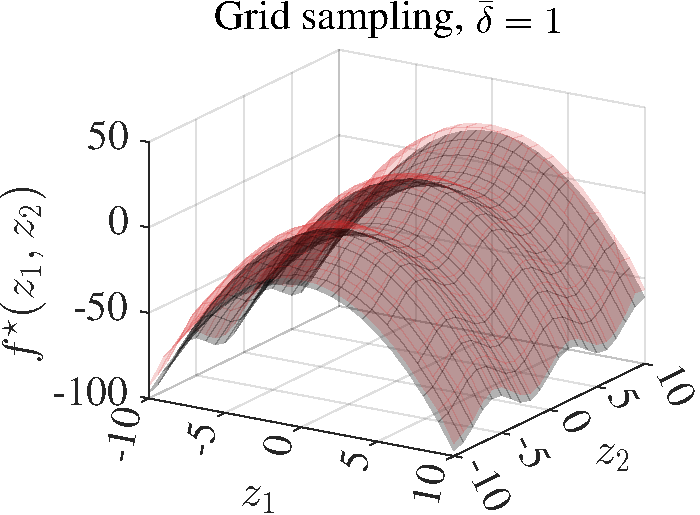
\includegraphics[scale=0.4]{../images/chap2_numex_ex1_grid_1.pdf} \hspace{5pt}
	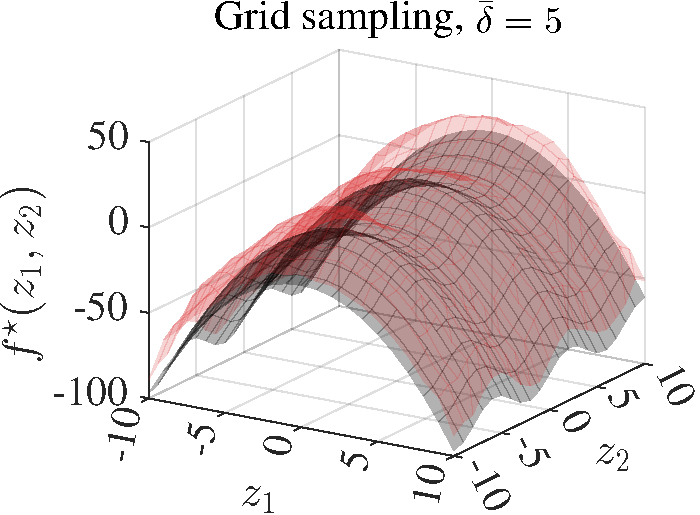
\includegraphics[scale=0.4]{../images/chap2_numex_ex1_grid_5.pdf} \\[13pt]
	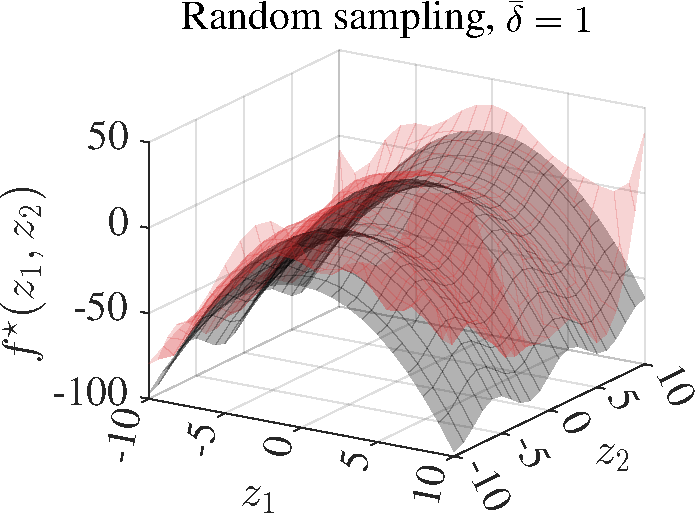
\includegraphics[scale=0.4]{../images/chap2_numex_ex1_rnd_1.pdf} \hspace{5pt}
	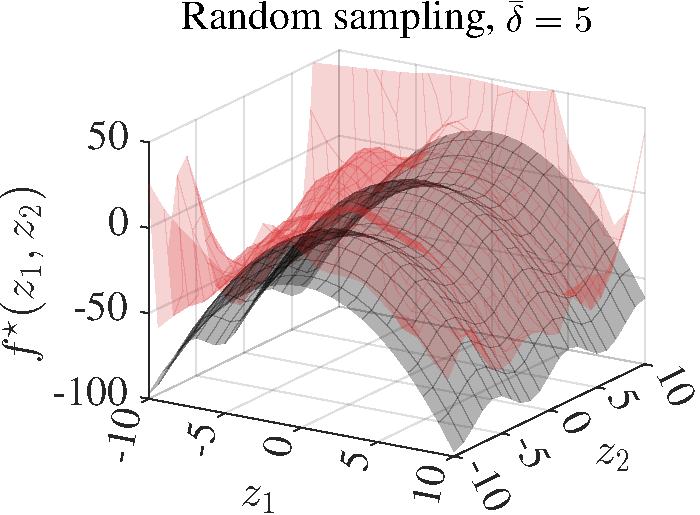
\includegraphics[scale=0.4]{../images/chap2_numex_ex1_rnd_5.pdf} 
	\caption{The ground-truth (black) and the optimal upper bound C$(x)$ (red) with $100$ data-points and different sampling methods and noise levels.}
	\label{fig.numex_ex1_3d}
	\vspace{15pt}
	\includegraphics[scale=0.4]{../images/chap2_numex_ex1_slice_grid_1.pdf} \hspace{5pt}
	\includegraphics[scale=0.4]{../images/chap2_numex_ex1_slice_rnd_1.pdf} 
	\caption{The ground-truth (solid black) sliced at $z_1 = -3$, the optimal bounds (red) and the sub-optimal bounds (dashed black).}
	\label{fig.numex_ex1_2d}
\end{figure}

It is desirable to have tight bounds $\bar\delta$ and $\Gamma$ in order to reduce conservativeness. This is however not possible in most practical applications where one has to estimate those quantities from data alone. To investigate the sensitivity of the resulting bounds with respect to those parameters, $\bar\delta$ and $\Gamma$ were varied to build

\begin{landscape}
	\vspace{30pt}
	\begin{table}
		\centering
		\caption{Noise uniformly sampled from $-1\leq \delta \leq 1$. 100 data-points were collected from the ground-truth \eqref{eq:ex1_gtfunc} in an equidistant grid (grid) or randomly following a uniform distribution (rnd). The table shows the average distance between the upper and lower bounds in the optimal (opt) and sub-optimal (sub) cases with various noise bounds $\bar\delta$ and RKHS norm estimates $\Gamma$.}
		\label{tab.numex_ex1_delta1}
		%\begin{tabular}{| c c || c | c | c || c | c | c || c | c | c ||} 
		\begin{tabular}{c c c c c c c c c c c } 
			%\hline
			\cmidrule[.15em](l{\tabcolsep}r{\tabcolsep}){1-11}
			\multicolumn{2}{ r }{$\Gamma$} & \multicolumn{3}{c}{1200}  & \multicolumn{3}{c}{1800} & \multicolumn{3}{c}{2400}\\
			%\hline
			\cmidrule[.05em](l{\tabcolsep}r{\tabcolsep}){2-11}
			\multicolumn{2}{r}{$\bar\delta$} & 1 & 1.5 & 2  & 1 & 1.5 & 2 & 1 & 1.5 & 2  \\
			%\hline \hline
			\cmidrule[.15em](l{\tabcolsep}r{\tabcolsep}){2-11}
			\multirow{3}{*}{\rotatebox[origin=c]{90}{\hspace{13pt}grid}} & opt & 6.21 & 8.35 & 10.34 &   7.45  & 9.75 & 11.90 & 8.50 & 10.94 & 13.20  \\
			\cmidrule[.05em](l{\tabcolsep}r{\tabcolsep}){2-11}
			& sub & 11.07  & 15.60 & 20.13   & 11.70  & 16.23 & 20.76 & 12.36  & 16.89 & 21.42  \\
			%\hline \hline
			\cmidrule[.15em](l{\tabcolsep}r{\tabcolsep}){2-11}
			\multirow{3}{*}{\rotatebox[origin=c]{90}{\hspace{14pt}rnd}} & opt & 14.62  & 19.02 & 22.89  & 18.05  & 23.08 & 27.51 & 20.85  & 26.39 &  31.26 \\
			%\cline{2-11}
			\cmidrule[.05em](l{\tabcolsep}r{\tabcolsep}){2-11}
			& sub & 64.78  & 93.99 & 123.20  & 65.91  & 95.12 & 124.33 & 67.07  & 96.28 & 125.49  \\
			%\hline \hline
			\cmidrule[.15em](l{\tabcolsep}r{\tabcolsep}){1-11}
		\end{tabular}
	\end{table}
	%
	\begin{table}
		\centering
		\caption{Noise uniformly sampled from $-5\leq \delta \leq 5$. 100 data-points were collected from the ground-truth \eqref{eq:ex1_gtfunc} in an equidistant grid (grid) or randomly following a uniform distribution (rnd). The table shows the average distance between the upper and lower bounds in the optimal (opt) and sub-optimal (sub) cases with various noise bounds $\bar\delta$ and RKHS norm estimates $\Gamma$.}
		\label{tab.numex_ex1_delta5}
		\begin{tabular}{c c c c c c c c c c c} 
			\cmidrule[.15em](l{\tabcolsep}r{\tabcolsep}){1-11}
			\multicolumn{2}{r}{$\Gamma$} & \multicolumn{3}{c}{1200}  & \multicolumn{3}{c}{1800} & \multicolumn{3}{c}{2400}\\
			\cmidrule[.05em](l{\tabcolsep}r{\tabcolsep}){2-11}
			\multicolumn{2}{r}{$\bar\delta$} & 5 & 7.5 & 10  & 5 & 7.5 & 10 & 5 & 7.5 & 10  \\
			\cmidrule[.15em](l{\tabcolsep}r{\tabcolsep}){2-11}
			\multirow{3}{*}{\rotatebox[origin=c]{90}{\hspace{13pt}grid}} & opt & 20.29 & 28.57 & 36.39 & 22.54  & 31.31 & 39.58 & 24.41 & 33.56 & 42.17  \\
			\cmidrule[.05em](l{\tabcolsep}r{\tabcolsep}){2-11}
			& sub & 49.15  & 71.79 & 94.44  & 49.81 & 72.46 & 95.11 & 50.48  & 73.13 & 95.78  \\
			\cmidrule[.15em](l{\tabcolsep}r{\tabcolsep}){2-11}
			\multirow{3}{*}{\rotatebox[origin=c]{90}{\hspace{14pt}rnd}} & opt & 39.95  & 53.43 & 65.41  & 47.00  & 62.15 & 75.57 & 52.76  & 69.32 & 83.89  \\
			\cmidrule[.05em](l{\tabcolsep}r{\tabcolsep}){2-11}
			& sub & 312.44  & 458.51 & 604.57  & 313.61   & 459.68 & 605.74 &  314.79 & 460.85 & 606.91  \\
			\cmidrule[.15em](l{\tabcolsep}r{\tabcolsep}){1-11}
		\end{tabular}
	\end{table}
\end{landscape}

a total of 18 test scenarios, divided into two noise cases as shown in Tables~\ref{tab.numex_ex1_delta1} and \ref{tab.numex_ex1_delta5}. The figures are consistent in showing that the average width was not significantly affected by an increase in $\Gamma$. Analyzing the numbers from Table~\ref{tab.numex_ex1_delta1}, the width of the optimal envelope  increased on average by 34\% when augmenting $\Gamma$ from 1200 to 2400, and the width of the sub-optimal envelope increased on average by 5.2\%. Repeating the analysis on Table~\ref{tab.numex_ex1_delta5}, the optimal envelope showed an average width increase of 24\%, whereas the sub-optimal one, of 1.38\%. Despite the larger relative increase of the optimal bounds width, their absolute values were on average 3.45 times smaller than the sub-optimal ones in Table~\ref{tab.numex_ex1_delta1} and 5.79 times smaller in Table~\ref{tab.numex_ex1_delta5}, which exposes the degree of conservativeness of the latter approach.

\textbf{Example 2:} The next numerical experiment involves having the map \eqref{eq:ex1_gtfunc} as a constraint in a static optimization problem\footnote{Maximizing/minimizing a given objective under unknown constraints is typical in the field of real-time optimization, see e.g. \citep{chachuat2009adaptation}.}. Consider the following formulation
\begin{subequations}
	\label{eq:rto}
	\begin{align}
		\min_{z \in \mathbb{R}^2} & \quad (z_1-1)^2 + (z_2-5)^2  \\ 
		\text{\normalfont subj. to} & \ \; 
		f^\star(z) \le -10, \label{eq:rtocons}
	\end{align}
\end{subequations}
where the function $f^\star(z)$ given by \eqref{eq:ex1_gtfunc} is not explicitly known, but can be measured, evaluated. Samples were used to establish an upper bound $\text{C}(z)$ for $f^\star(z)$, hence providing an inner-approximation for the true feasible set of \eqref{eq:rto}. 

We considered the cases of having 64, 81 and 100 evaluations of $f^\star(z)$ affected by noise with $\bar\delta=1$ and, once more, the data were collected by means of a uniform random distribution and an equidistant grid. The same kernel function and RKHS norm estimate of $\Gamma=1200$ from Example~1 were used. In the surrogate optimization problems, \eqref{eq:rtocons} was replaced by $C(z)\le -10$. Optimizers $z^\star$ were computed by gridding the domain, and the results along with the estimated feasible sets (shaded areas) are shown in Figure~\ref{fig:constraints}. Notice how in some instances the set of feasible decisions is not connected. Thanks to Proposition~\ref{prop.decreasing}, the addition of new data-points can only relax the approximate formulation, hence reducing the found minimum.
Indeed, the obtained solutions for the approximate problems were $13.21$, $11.36$ and $10.96$, respectively with $64$, $81$ and $100$ samples taken randomly. When employing a grid, the figures were $10.67$, $8.48$ and $7.67$. The solution of the real problem, i.e., the one with the ground-truth constraint, is $5.69$.

\begin{figure*}[t]
	\centering
	\includegraphics[scale=0.25]{../images/chap2_numex_ex2_gt.pdf} \\
	\includegraphics[scale=0.25]{../images/chap2_numex_ex2_res.pdf}
	\caption{Solutions and feasible sets (shaded areas) of the surrogate optimization problems, i.e., \eqref{eq:rto} with the constraint replaced by its optimal upper bound C$(x) \leq -10$. The individual solutions are denoted by the yellow, orange and red triangles and stars. The true optimum is depicted as a black star.}
	\label{fig:constraints}
\end{figure*}

\textbf{Example 3:} In this example, UQ will be used to verify the safety of a sequence of control actions driving a dynamical system. As opposed to the grid-based and randomized sampling methods used in the previous examples, the dynamics will be taken into account and data will be gathered directly from trajectories.

Consider a continuous stirred-tank reactor (CSTR) described by the continuous-time differential equations \begin{subequations}
	\begin{align}
		\dot{c}_A(t) &= u(t)(c_{A0}-c_A(t)) - \rho_1 c_A(t) - \rho_3 c_A^2(t)  \\ 
		\dot{c}_B(t) &= -u(t)c_B(t) + \rho_1 c_A(t) - \rho_2 c_B^2(t)
	\end{align}
\end{subequations}
where $c_A$ and $c_B$ denote respectively the concentrations of cyclopentadiene and cyclopentenol, whereas $u$ represents the feed inflow of cyclopentadiene. The parameters are $\rho_1 = \rho_2 = 4.1 \times 10^{-3}$ h$^{-1}$, $\rho_3 = 6.3 \times 10^{-4}$ h$^{-1}$, $c_{A0} = 5.1$ mol/l. The system is subject to the constraints $1 \leq c_A \leq 3$, $0.5 \leq c_B \leq 2$, $3 \leq u \leq 25$, and is sampled at a rate of $1/30~$Hz. The goal is to drive the states from a number of initial conditions to the reference values $c_A^{\text{ref}} = 2.14$, $c_B^{\text{ref}} = 1.09$. To achieve this objective, a finite-horizon optimal control problem (OCP) with horizon $N=8$ was formulated employing a standard quadratic cost with a larger terminal weight but no terminal set constraint. The OCP relied on a KRR nominal model learned from data and no uncertainty quantification, i.e., relied on certainty equivalence.

\begin{figure}[t]
	\centering
	\includegraphics[scale=0.4]{../images/chap2_numex_ex3_phase_subopt.pdf} \hspace{5pt}
	\includegraphics[scale=0.4]{../images/chap2_numex_ex3_phase_opt.pdf} 
	\caption{A comparison between the optimal bounds (blue) and the closed-form sub-optimal ones (green). The 2D ground-truth was sliced at $z_1 = -3$ and is shown in dashed black.}
	\label{fig:ex3_phase}
	\vspace{15pt}
	\includegraphics[scale=0.4]{../images/chap2_numex_ex3_time_subopt.pdf} \hspace{5pt}
	\includegraphics[scale=0.4]{../images/chap2_numex_ex3_time_opt.pdf}
	\caption{The ground-truth (black) and the upper optimal bound C$(x)$ (blue) with $100$ data-points. Two noise levels are considered, $\bar\delta = 1$ and $\bar\delta = 5$, and two sampling strategies, an equidistant grid and random uniform sampling.}
	\label{fig:ex3_time}
\end{figure}

To verify if computed OCP control actions would not lead to the system violating constraints, we employed our kernelized UQ technique. First, the problem was broken down into several steps: the 1-step ahead analysis, the 2-step ahead analysis, and so on. The datasets associated with each step are composed of initial states and sequences of control actions to form $x_i$, and the final state to form $y_i$ (this multi-step approach is the same as the one explained in Section~\ref{sec.kpc}). The squared-exponential kernel was used throughout the whole process and the various lengthscales were selected through a 5-fold cross-validation process based on 400 samples (see Section~\ref{sec.appendix_hyerparams}). The same batch of data were exploited to estimate the different RKHS norms $\Gamma$ following the procedure of Section~\ref{sec.appendix_estimating_rkhs_norms}. The obtained lower estimates were then augmented to account for possible unseen complexity. Distinct datasets were gathered to compute the bounds by starting the system at $800$ initial conditions and solving OCP from those locations. We highlight that, as there are two states and one control variable, the domain of the function mapping the initial condition to the 8-th step ahead state has dimension 10, hence justifying the need for a large dataset. The noise affecting the measurements was drawn uniformly from the interval $-0.05$ to $0.05$, and a bound of $\bar \delta = 0.06$ was used.

The optimal bounds \eqref{eq.P1case1} and the sub-optimal ones \eqref{eq.uniformBound2} were employed to define robust confidence sets for each time-step. These are guaranteed to contain the true system evolution, the ground-truth, as illustrated by the phase portrait and the bounding boxes in Figure~\ref{fig:ex3_phase}. Based solely on the sub-optimal approach, one would certify three out of four control sequences as the one confidence set in the lower right portion of the space extends beyond the state constraints. Nevertheless, by using the optimal bounds we can conclude that no violation would occur as all confidence sets are completely within the feasible region. A time-domain view of that particular trajectory is shown in Figure~\ref{fig:ex3_time}. It is important to underline that both approaches are based exactly on the same information (datasets, noise bounds and RKHS norm bounds), and only differ in the way they are computed.

\textbf{Example 4:} The continuous-time angular dynamics of a pendulum with a rigid rod can be described by $\dot x_1 = x_2$, $\dot x_2 = (g/l)\sin(x_1) - (\nu/(ml^2)) x_2 + (1/(m l^2)) u$, where $x_1$ is its angular position, $x_2$ its angular velocity, and $u$ the torque applied to it. The parameters are: $m = 0.15$ the mass of the pendulum, $l = 0.5$ the length of the rod, $g = 9.81$ the gravitational constant, and $\nu = 0.1$ a constant for the friction model. Let the constraints be $\vert x_1 \vert \leq 3$, $\vert x_2 \vert \leq 1$, and the input be limited to $\vert u \vert \leq 1$. We selected a prediction horizon of $N=4$ and collected $D=100$ uniformly random data-points for each of the eight regression tasks. The noise was drawn randomly from a uniform distribution with bound $\bar \delta = 0.01 \, \textbf{1}$, where $\textbf{1} \in \mathbb{R}^D$ is a vector of ones. Similarly to the previous example, we used a squared-exponential kernel with increasing lengthscales and employed an augmentation factor of $300\%$ on the nominal predictor norms to estimate the $\Gamma$ constants. The sampling and control period was $0.2$~seconds. We compared KPC against \textit{nominal} kernel-MPC, i.e., a certainty equivalence approach where the state-constraints were imposed directly on the nominal predictions \eqref{eq.KPCnominal}. In the latter case, uncertainty was not quantified and the confidence sets were not present. The cost used in both formulations was a positive definite function of the states and control inputs, and included a terminal penalty term. 

Predictions and the system angular velocity evolution from two different initial conditions are shown in Figure~\ref{fig.PENDULUM}. As can be seen from the plots, imposing the state-constraints on the nominal model predictions was not sufficient to guarantee safety as the closed-loop system behavior violated the $x_2 \geq -1$ restriction. On the other hand, since KPC quantified and incorporated the associated uncertainty into the optimization problems, the constraints were satisfied. The error bars on the right plot show the all predictions and uncertainty values at each step in the form of error bars. Note that the safety constraints were active at multiple points in time. 

\begin{figure}[t]
	\centering
	\includegraphics[scale=0.25]{../images/chap2_numex_ex4_A.pdf}
	\includegraphics[scale=0.25]{../images/chap2_numex_ex4_B.pdf}
	\includegraphics[scale=0.25]{../images/chap2_numex_ex4_C.pdf}
	\caption{A comparison between the optimal bounds (blue) and the closed-form sub-optimal ones (green). The 2D ground-truth was sliced at $z_1 = -3$ and is shown in dashed black.}
	\label{fig.PENDULUM}
\end{figure}
	
%%%%%%%%%%%%%%%%%
%%%%%%%%%%%%%%%%%
% Appendices
%%%%%%%%%%%%%%%%%
%%%%%%%%%%%%%%%%%

\section{Conclusions and outlook}

In this first part of the thesis, we introduced and developed a novel way of quantifying the out-of-sample uncertainty of the values of an unknown function. The framework was built around kernels, their RKHS spaces, and a bounded measurement noise assumption from which no statistical information is known. Optimal hard upper and lower bounds were then derived, being computable through convex optimization. Closed-form conservative approximation schemes were given to be used in time-constrained scenarios. Some properties of the optimal and sub-optimal approaches were derived and their sensitivity to the internal parameters (the RKHS norm estimate and the noise bound) were studied. The techniques were finally employed to solve a number of problems ranging from a direct function bounding one, to solving an optimization problem with unknown constraints, to certifying optimal control actions.

We envision multiple future investigations and extensions of the theory presented in this chapter. First, additional properties of the optimal bounds could be established, in particular, although we have not had the time to prove it, we suspect the upper and lower envelopes C$(x)$ and B$(x)$ to be continuous and piece-wise smooth whenever the base kernel $k$ is smooth. Deriving this result would likely involve studying the solution set and the value function of the parametric program \eqref{eq.P1case1}.  One necessary extension to allow for the learning of dynamical systems from trajectories, and not resorting to multi-step ahead models, is to consider uncertainty in $x$ itself. This would call of course for robust parametric programming to be employed. Finally, on the application side, the KPC framework presented in Section~\ref{sec.kpc} guarantees constraint satisfaction, but can be rather challenging to implement in practice due to the use of multiple models. Long prediction horizons are generally desirable to favor stability, however, this requires more models to be trained in higher dimensional spaces since longer and longer control sequences are incorporated into the feature vector. Estimating hyperparameters and filling the space with data then become difficult tasks in such scenarios, limiting therefore KPC to short prediction horizons. To eliminate some of these difficulties, a different approach to kernel-based predictive control could be adopted, that of optimism. Instead of being robust against all possible ground-truth dynamics, one could pick a dynamic that is consistent with the historical data and complexity bound, the most convenient one. As the system is operated and more information is gathered, the set of possibilities is reduced and the adopted dynamic would be more consistent with the true unknown dynamics. We believe that, based on recent regret bounds for kernelized global optimization, convergence rates could be derived for the iterative performance improvement of this scheme and bounds could be established for the constraint violation frequency.

\section{Appendices}

\subsection{Estimating kernel hyperparameters}
\label{sec.appendix_hyerparams}

Kernel functions typically feature a number of internal constants that need to be specified by the user, the so-called \textit{hyperparameters}. Although some theoretical properties remain insensitive to the final choice of hyperparameters\footnote{For instance, the squared-exponential kernel is universal (Definition~\ref{def.universal_kernel}) regardless of the its lengthscale value. On the other hand, it is known that if $k_\ell$ is a squared-exponential kernel with lengthscale $\ell$, then $\rkhs_{k_{\ell1}}$... \mycomment{cite Ingo's book}}, the numerical stability and real-world performance of kernel algorithms highly depend on the tuning of these numbers \citep{fasshauer2011positive}. 

One popular approach to optimizing kernel hyperparameters is to consider the log marginal likelihood objective of a Gaussian process with Gaussian measurement noise, and apply a gradient-based numerical algorithm to it \citep[§5.4.1]{williams2006gaussian}. This amounts to solving a smooth, unconstrained non-convex optimization problem to local optimality.  Two appealing ... of this approach are the continuous nature of the search and the inherent regularization properties of the objective, known to combat overfitting. 

Bayesian optimization (BayesOpt) is another widely adopted methodology to fine-tune hyperparameters against a pre-specified objective function \citep{snoek2012practical,shahriari2015taking}. BayesOpt operates on pairs of hyperparameters and their associated objective function values, and constructs a model for their unknown relationship. Next, a so-called \textit{acquisition function} based on the model is then employed to tell bad hyperparameters from promising ones \citep{wilson2018maximizing}. A new set of parameters is finally chosen to be experimented with and its performance is measured. This new piece of information is incorporated into the dataset and the process is repeated until some termination criterion is reached. Interestingly, the most popular model class used when reconstructing the aforementioned unknown relationship is Gaussian process, which is itself based on kernels whose own hyperparameters have to be set by the users.

Lastly, we could also mention the different flavors of cross-validation (CV). The procedure builds an estimate of how suitable a set of hyperparameters are by evaluating the resulting model performance on unseen data. More specifically, it consists in shuffling and splitting the available data into batches, say $N$; making use of $N-1$ batches to define the model and the last one to assess its performance; the process is repeated $N$ times rotating the batches and yielding $N$ performance measures, which could be combined through averaging for instance. By following this algorithm, the most suitable hyperparameter value could be found from a predefined list of possible values. An extreme version of CV is leave-one-out cross-validation (LOOCV), whereby a $d$-sample dataset is divided into $d$ batches. Finally, note that the log marginal likelihood itself could be a valid performance objective within CV \citep[§5.4.2]{williams2006gaussian}.

\subsection{Estimating RKHS norms}
\label{sec.appendix_estimating_rkhs_norms}

Members $f \in \rkhs$ are either finite weighted sums of partially evaluated kernels $k(x,\cdot)$ or limits of sequences of such sums (see Section~\ref{sec.formalism_of_kernels}). Assume $f$ enjoys a finite expansion of $N$ terms, then
\begin{align}
	\Vert f \Vert_\rkhs^2 &= \langle f, f \rangle_\rkhs \label{eq.rkhs_norm_eq1} \\
	&= \left\langle \sum_{i=1}^N \alpha_i k(x_i,\cdot), \sum_{i=1}^N \alpha_i k(x_i,\cdot) \right\rangle_\rkhs \label{eq.rkhs_norm_eq2} \\
	&= \alpha^\top K_{XX} \alpha \label{eq.rkhs_norm_eq3}
\end{align}
where \eqref{eq.rkhs_norm_eq1} is the RKHS norm definition, \eqref{eq.rkhs_norm_eq2} is the inner-product definition, and \eqref{eq.rkhs_norm_eq3} follows from the inner-product linearity and from the reproducing property of kernels (see \eqref{eq.reproducing_property}). As a result, the norm $\Vert f \Vert_\rkhs$ can be exactly and easily computed as long as we have at hand the weights $\alpha$ that define $f$.

In practice, it is hard to imagine a situation where the coefficients $\alpha$ would be known for a given physical system. Suppose however that we have a dataset at hand $\{(x_i,f_{x_i})\}\}_{i=1}^n$, where $f_{x_i} = f(x_i)$. The inputs $x_i$ need to be pairwise-distinct. Assume that $k$ is SPD and consider the function $s_n(x) := \sum_{i=1}^n \alpha_i k(x_i,x)$, $\alpha = K_{XX}^{-1} f_X$, which reproduces our dataset at every input, i.e., $s_n(x_i) = f_{x_i}$. According to the well-known optimal recovery property \cite[§8.3]{iske2018approximation}, $s_n$ not only interpolates the dataset, but also attains a minimum RKHS norm while doing so  (Proposition~\ref{prop.MNI}) and, moreover, $\Vert s_n \Vert_\rkhs \leq \Vert f \Vert_\rkhs$ for any number of samples $n$. In view of the quadratic form \eqref{eq.rkhs_norm_eq3}, it is evident that for any new pair $(x_{n+1},f_{x_{n+1}})$ added to the dataset, $\Vert s_{n+1} \Vert_\rkhs \geq \Vert s_n \Vert_\rkhs$ holds. One can finally show that if samples are acquired in such a way to fill the domain, then $\Vert f \Vert_\rkhs$ is the least upper bound of the $\Vert s_n \Vert_\rkhs$ sequence and, from the monotone convergence theorem, $\Vert s_n \Vert_\rkhs \rightarrow \Vert f \Vert_\rkhs$ is guaranteed.

The discussion above showed that the RKHS norm $\Vert f \Vert_\rkhs$ can indeed be estimated from below from samples $\{(x_i,f_{x_i})\}_{i=1}^n$. This is done by simply evaluating the norm of the interpolant for which we know the weights $\alpha$
\begin{equation}
\Vert s_n \Vert_\rkhs^2 = \alpha^\top K_{XX} \alpha = f_{X}^\top K_{XX}^{-1} f_{X}
\end{equation}
The more samples we have, the closer the quadratic form will be from the target value $\Vert f \Vert_\rkhs$. Consider the example below for observations on how the estimation process unfolds in a practical scenario.

\begin{figure}[b]
	\centering
	%\hspace{1pt}
	\includegraphics[scale=1]{../images/norm_est.pdf} 
	\includegraphics[scale=1]{../images/norm_value.pdf} %\hspace{8pt}
	\caption{Estimating the RKHS norm of a function (left) from samples. The norm value of the MNI interpolant for an increasing number of samples (right) is shown to gradually approach the RKHS norm of the ground-truth.}
	\label{fig.appendice_norm_estimation}
\end{figure}

Let $k:\mathbb{R}\times \mathbb{R} \rightarrow \mathbb{R}$ be the squared-exponential with lengthscale $\ell = 0.5$. A member $f \in \mathcal{H}$ of its RKHS is shown in Figure~\ref{fig.appendice_norm_estimation} (left), being composed of $100$ partially evaluated kernels whose centers and weights were randomly generated. The exact $\Vert f\Vert_\rkhs$ value was computed through \eqref{eq.rkhs_norm_eq3}, yielding $\Vert f\Vert_\rkhs = 11.24$. Next, the same quantity was estimated through data simply drawn randomly from the domain, following a uniform distribution. The associated $\Vert s_n \Vert_\rkhs$ from $n=1$ to $60$ is shown in Figure~\ref{fig.appendice_norm_estimation} (right). At around $n=42$, the lower estimate is seen to have essentially reached the $\Vert f \Vert_\rkhs$ level, capturing all the complexity there was to capture. Lastly, we selected a subset of only six of the previously samples points, those closer to some of the function peaks, and computed the associated interpolant norm. The value of 10.02 was obtained, i.e., 89\% of $\Vert f \Vert_\rkhs$, illustrating that a few well-located samples can already offer us a reasonable measure of the unknown ground-truth RKHS norm.

Up to this point, only noiseless samples were consider. Suppose now the data come in the form $\{(x_i,y_i)\}_{i=1}^n$ with $x_i$ pairwise distinct and $y_i=f(x_i) + \delta_i$. Let the additive noise be bounded by some known value $\bar \delta \geq |\delta_i|$ for all $i$. Since we do not have access to the evaluations of $f$ anymore, $\Vert s_n \Vert_\rkhs$ cannot be computed. If we naively interpolate the data with the model $\tilde s_n(x) := \sum_{i=1}^n \alpha_i k(x_i,x)$, $\alpha = K_{XX}^{-1} y$, the resulting norm $\Vert \tilde s_n \Vert_\rkhs^2 = y^\top K_{XX}^{-1}y$ can be either larger or smaller than its noise-free counterpart. The mismatch between the two will depend on how each $\delta_i$ will disturb the samples, and its maximum effects can be exactly computed.

\begin{proposition}
	Let $\{(x_i,y_i)\}_{i=1}^n$ be such that $x_i$ are pairwise distinct and $y_i = f(x_i) + \delta_i$ with $\bar \delta \geq |\delta_i|$ for all $i$. Let $s_n$ and $\tilde s_n$ be respectively the models interpolating the noise-free $f_X$ and the noisy $y$ values of $f$, i.e., $s_n(x) = \sum_{i=1}^n \alpha_i k(x_i,x)$, $\alpha = K_{XX}^{-1} f_X$ and $\tilde s_n(x) = \sum_{i=1}^n \alpha_i k(x_i,x)$, $\alpha = K_{XX}^{-1} y$. It then holds that
	\begin{equation}
		\nabla \leq \Vert \tilde s_n \Vert_\rkhs^2 - \Vert s_n \Vert_\rkhs^2 \leq \Delta
	\end{equation}
	where $\Delta$ and $\nabla$ denote respectively the maximum and minimum of $-\delta^\top K_{XX}^{-1} \delta + 2y^\top K_{XX}^{-1} \delta$ over $\delta$, subject to $|\delta| \leq \bar \delta$.
	\label{prop.norms_mismatch}
\end{proposition}

Calculating $\Delta$ amounts to solving a convex optimization problem since it is the maximum of a strictly concave function, whereas $\nabla$ is not as simple.

%\begin{proposition}
%	Let all assumption listed in Proposition~\ref{prop.norms_mismatch} hold and, additionally, $\delta$ be a random vector with $\mathbb{E}(\delta) = \mu$ and $\mathbb{V}(\delta) = \Sigma$, then
%	\begin{equation}
%		\mathbb{E}(\Vert \tilde s_n \Vert_\rkhs^2 - \Vert s_n \Vert_\rkhs^2) = \mu^\top K_{XX}^{-1} \mu + \text{Tr}(K_{XX}^{-1}\Sigma) + 2y^\top K_{XX}^{-1} \mu
%	\end{equation}
%	Moreover, if $\delta$ follows a uniform distribution $\mathcal{U}(-\bar \delta, \bar \delta)$, then $\mathbb{E}(\Vert \tilde s_n \Vert_\rkhs^2 - \Vert s_n \Vert_\rkhs^2) = \dots$
%	\label{prop.expected}
%\end{proposition}

\subsection{Auxiliary definitions}
\label{sec.auxiliary_definitions}

Recall that $n_1, n_2, \dots, n_d$ are the number of outputs available at the input locations $x_1,x_2,\dots,x_d$. Let $\Lambda$ be the matrix of size $(\sum_i n_i) \times d$ defined as
\begin{equation}
	\Lambda :=
	\begin{bmatrix}
		\bm{1}_{n_1} & \bm{0}_{n_1} & \bm{0}_{n_1} & \cdots & \bm{0}_{n_1} \\
		\bm{0}_{n_2} & \bm{1}_{n_2} & \bm{0}_{n_2} & \cdots & \bm{0}_{n_2} \\
		\vdots & \vdots & \vdots & \ddots & \vdots \\ 
		\bm{0}_{n_d} & \bm{0}_{n_d} & \bm{0}_{n_d} & \cdots & \bm{1}_{n_d} 
	\end{bmatrix}
\end{equation}
where $\bm{1}_{n_i}$ and $\bm{0}_{n_i}$ are respectively column vectors of ones and zeros of size $n_i$. If only a single output is available at every input, $\Lambda$ simplifies to an identity matrix.

The column vector $f_X$ is made of function evaluations $f(x_i)$, which are repeated whenever multiple outputs are available at the same input location $x_i$. More concretely, $f_X := \Lambda \begin{bmatrix} f(x_1) & \dots & f(x_d) \end{bmatrix}^\top$.

\subsection{Proofs}
\label{sec.selected_derivations}

In this section we provide proofs for all the propositions found throughout the chapter that were left unproven.

\begin{my_proof}
	\textbf{Proof of Proposition~\ref{prop.complex_constraint_always_active}:}
	It follows from the objective being linear and only sensitive to $c_x$ and from reformulating \eqref{eq.P1constrA}. More concretely, we use the matrix inversion lemma and the definition of $P_X(x)$ to re-write the complexity constraint as
	\begin{subequations}
		\begin{align}
			\begin{bmatrix}
				c \\
				c_x
			\end{bmatrix}^\top 
			\begin{bmatrix}
				K_{XX} & K_{Xx} \\
				K_{xX } & k(x,x)
			\end{bmatrix}^{-1} 
			\begin{bmatrix}
				c \\
				c_x
			\end{bmatrix} & \leq \Gamma^2 
		   \label{eq.appendix_complex_constr_terms1}
		   \\
			%
			\Leftrightarrow \;
			c^\top K^{-1}_{XX} c
			+
			P_{X}^{-2}(x) \, \left( c^\top K_{XX}^{-1} K_{Xx} - c_x \right)^2 
			&\leq \Gamma^2 
			\label{eq.appendix_complex_constr_terms}
		\end{align}
	\end{subequations}
	Note that $P_X^{-2}(x) > 0$ since $P_X(x) > 0$ for any $x$ not in $X$ \citep{karvonen2022error}. As a result, we see that \eqref{eq.appendix_complex_constr_terms} depends quadratically on $c_x$. Therefore, for any feasible $(c, c_x)$ such that \eqref{eq.appendix_complex_constr_terms1} is inactive, there exists $ \tilde c_x := c_x + \varepsilon, \varepsilon > 0$ such that $(c,\tilde c_x)$ attains a higher objective while satisfying the constraints.
\end{my_proof}

\begin{my_proof}
	\textbf{Proof of Proposition~\ref{prop.smallWidth}:}
	Follows from $\text{C}(x_i) \geq \text{B}(x_i)$, $\text{C}(x_i) \leq y_{i,j} + \bar \delta$ and $\text{B}(x_i) \geq y_{i,j} - \bar \delta$ for any $i=1,\dots,d$ and any $j=1,\dots,n_i$. 
\end{my_proof} 

\begin{my_proof}
	\textbf{Proof of Proposition~\ref{prop.decreasing}:}
	Denote by $\mathds{P}1_1$ the problem solved with $D_1$ and decision variables $\begin{bmatrix} c & c_x \end{bmatrix}$. Similarly, $\mathds{P}1_2$ is associated with the dataset $D_2$ and the decision variables $\begin{bmatrix} c & c_x & c_z \end{bmatrix}$, where $c_z$ are due to the additional input in $D_2$. Since $D_2$ contains all members of $D_1$, the $\infty$-norm constraint of $\mathds{P}1_2$ can be recast as that of $\mathds{P}1_1$ and an additional constraint for $c_z$ and the new outputs. Let $\mathds{X}  := X \cup \{x\}$, $\bar c := \begin{bmatrix} c^\top c_x \end{bmatrix}^\top$ and $z := x_{d+1}$ be shorthand variables to ease notation. The complexity constraint of $\mathds{P}1_2$ is then
	
	\begin{subequations}
		\begin{align}
			\begin{bmatrix}
				\bar c \\
				c_z
			\end{bmatrix}^\top 
			\begin{bmatrix}
				K_{\mathds{X} \mathds{X} } & K_{\mathds{X}  z} \\
				K_{z \mathds{X} } & k(z,z)
			\end{bmatrix}^{-1} 
			\begin{bmatrix}
				\bar c \\
				c_z
			\end{bmatrix} & \leq \Gamma^2 \\
			%
			\overset{(i)}{\Leftrightarrow}
			\bar c^\top K_{\mathds{X} \mathds{X} }^{-1} \bar c +
			P_{\mathds{X} }^{-2}(z) \, 
			%\begin{bmatrix}
			%	\bar c \\
			%	c_z
			%\end{bmatrix}^\top
			%\begin{bmatrix}
			%	K_{\bar X \bar X}^{-1} K_{\bar X z} \\
			%	-1
			%\end{bmatrix}
			\left\|
			\begin{bmatrix}
				K_{\mathds{X} \mathds{X} }^{-1} K_{\mathds{X} z} \\
				-1
			\end{bmatrix}
			\begin{bmatrix}
				\bar c \\
				c_z
			\end{bmatrix}\right\|_2^2
			& \leq \Gamma^2 \\
			%
			\overset{(ii)}{\Leftrightarrow} \;
			\begin{bmatrix}
				c \\
				c_x
			\end{bmatrix}^\top 
			\begin{bmatrix}
				K_{XX} & K_{Xx} \\
				K_{xX} & k(x,x)
			\end{bmatrix}^{-1} 
			\begin{bmatrix}
				c \\
				c_x
			\end{bmatrix} \label{eq.tightenedConstr}%\\\notag
			+
			P_{\mathds{X} }^{-2}(z) \, \left( \bar c^\top K_{\mathds{X} \mathds{X} }^{-1} K_{\mathds{X} z} - c_z \right)^2 
			&\leq \Gamma^2 
		\end{align}
		\label{eq.quadraticDecomp}
	\end{subequations}
	where the matrix identity \eqref{eq.matrix_inv_lemma} was used in $(i)$ along with $P^2_{\mathds{X} }(z) = k(z,z) - K_{z \mathds{X} } K_{\mathds{X} \mathds{X} }^{-1} K_{\mathds{X} z}$. In $(ii)$, the definitions of $\bar c$ and $\mathds{X} $ were used. Thanks to $P_{\mathds{X} }(z) \geq 0, \forall z$ \citep{karvonen2022error} and the quadratic term multiplying it, we conclude that for any choice of the decision variable $c_z$, \eqref{eq.tightenedConstr} is a tightened version of the complexity constraint of $\mathds{P}1_1$. As a result, the maximum of $\mathds{P}1_2$ is lower or equal than that of $\mathds{P}1_1$. 
\end{my_proof}

\begin{my_proof}
	\textbf{Proof of Proposition~\ref{prop.dual_problem}:}
	Consider the case $x \not\in X$. Let $z := \begin{bmatrix} c^\top & c_x\end{bmatrix}^\top$, $a := \begin{bmatrix} \textbf{0}^\top & 1\end{bmatrix}^\top$, $A := \begin{bmatrix} \textbf{I} & \textbf{0}\end{bmatrix}$. The Lagrangian of $\mathds{P}1$ is
	\begin{equation}
		\label{eq.lagrangianP2}
		\mathcal{L}(z,\lambda,\beta,\gamma) = a^\top z - \lambda (z^\top K_{\mathds{X}\mathds{X}}^{-1}z - \Gamma^2) - \beta^\top(\Lambda Az - \mathsf{y} - \bar \delta \textbf{1})- \gamma^\top(\mathsf{y} -\Lambda Az - \bar \delta \textbf{1})
	\end{equation}
	where $K_{\mathds{X}\mathds{X}}$ denotes the kernel matrix evaluated at $X \cup \{x\}$. Suppose $\lambda > 0$. Computing $\nabla_z\mathcal{L}(z^\star) = 0$ leads to
	$$z^\star = -\frac{1}{2\lambda}K_{\mathds{X}\mathds{X}} \left( A^\top \Lambda^\top (\beta - \gamma) - a \right).$$ 
	Note that $\beta$ and $\gamma$ cannot be simultaneously zero element-wise. Defining $\nu := \beta - \gamma$ and substituting $z^\star$ into \eqref{eq.lagrangianP2} gives the dual objective
	\begin{align}\notag
		g(\lambda,\nu) 
		=\;& \frac{1}{4\lambda} \nu^\top \Lambda A K_{\mathds{X}\mathds{X}} A^\top \Lambda^\top \nu + \left(\mathsf{y} - \frac{1}{2\lambda} \Lambda A K_{\mathds{X}\mathds{X}} a \right)^\top \nu \\
		&+ \bar \delta \Vert \nu \Vert_1 +  \frac{1}{4\lambda} a^\top K_{\mathds{X}\mathds{X}} a + \lambda \Gamma^2 \\\notag
		=\;& \frac{1}{4\lambda} \nu^\top \Lambda K_{XX} \Lambda^\top \nu + \left(\mathsf{y} - \frac{1}{2\lambda} \Lambda K_{Xx} \right)^\top \nu \\
		&+ \bar \delta \Vert \nu \Vert_1 +  \frac{1}{4\lambda} k(x,x) + \lambda \Gamma^2 \label{eq.dualDerivation}
	\end{align}

	where in the second equality the matrix $K_{\mathds{X}\mathds{X}}$ was expanded and the resulting terms were reorganized. Since $\beta,\gamma \in \mathbb{R}^{\tilde d}_{\geq 0}$ and $\nu = \beta - \gamma$ then $\nu$ is unconstrained.
	
	Now if $\lambda = 0$, the Lagrangian \eqref{eq.lagrangianP2} simplifies to
	$\mathcal{L}(z,\nu) = (a - A^\top \Lambda^\top \nu)^\top z + \nu^\top \mathsf{y} + \bar\delta \Vert \nu \Vert_1 \label{eq.lamZero}$, which is linear in $z$. Its supremum w.r.t. $z$ is only finite if $a = A^\top\Lambda^\top\nu$. Recalling the definitions of $a$, $A$ and $\Lambda$, one can see that $\nexists \nu$ that could satisfy the latter condition. Therefore, $\lambda = 0 \implies \sup_z \mathcal{L}(z,\lambda,\nu) = +\infty$, meaning that the dual problem is infeasible. As a conclusion, the Lagrangian dual of $\mathds{P}1$ in \eqref{eq.P2} is precisely $\mathds{D}1$ in \eqref{eq.dualProb}.
	
	Next, consider the case $x \in X$, $x = x_i$. The objective of $\mathds{P}1'$ can be written as $a^\top c$ with $a_i = 1$ and $a_n=0, n \neq i$. When deriving its Lagrangian, one obtains again \eqref{eq.lagrangianP2} with the simplifications: $z \leftarrow c$, $K_{\mathds{X}\mathds{X}} \leftarrow K_{XX}$ and $A \leftarrow \textbf{I}$. We proceed by analyzing the two scenarios for $\lambda$ as before. If $\lambda > 0$, the previous derivations apply, leading to the same the quadratic-over-linear objective \eqref{eq.dualDerivation}. However, if $\lambda = 0$, the Lagrangian becomes $\mathcal{L}(z,\nu) = (a -  \Lambda^\top \nu)^\top z + \nu^\top \mathsf{y} + \bar\delta \Vert \nu \Vert_1$, whose supremum w.r.t. $z$ is only finite if $a = \Lambda^\top \nu$. In contrast with the previous paragraph, this condition now can be satisfied. It is equivalent to $\nu_{i,1} + \dots + \nu_{i,n_i} = 1$, where the variables are all the multipliers associated with the $i$-th input location $x_i$. The resulting expression can be minimized analytically, yielding the minimum $\min_{j} y_{i,j} + \bar\delta$, i.e., the smallest output available at $x_i$ augmented by the noise bound. Finally, we conclude that the dual objective for $\mathds{P}1'$ is
	\begin{equation}
		g(\lambda,\nu) = 
		\begin{cases}
			\eqref{eq.dualDerivation}, & \text{if } \lambda > 0 \\
			\min_j y_{i,j} + \bar\delta, & \text{if } \lambda = 0
		\end{cases}
	\end{equation}
	
	As a last observation, a dual problem can also be derived for \eqref{eq.BofX}, calculating the lower part of the envelope. The formulation is analogous to \eqref{eq.dualProb}, assuming the form
		\begin{equation}
			\max_{\nu \in \mathbb{R}^{\tilde d}, \lambda > 0}\; -\frac{1}{4\lambda} \nu^\top \Lambda K_{XX} \Lambda^\top \nu - \left(\mathsf{y} + \frac{1}{2\lambda} \Lambda K_{Xx} \right)^\top \nu - \bar \delta \Vert \nu \Vert_1 - \frac{1}{4\lambda} k(x,x) - \lambda \Gamma^2
		\end{equation}
	Note that these are distinct objectives, not merely opposites. Therefore, two problems have to be solved to fully quantify the ground-truth uncertainty.
\end{my_proof} 

\begin{my_proof}
	\textbf{Proof of Proposition~\ref{prop.strong_duality}:}
	Consider the primal problem $\mathds{P}1$ and select $c = f^\star_X$ and $c_x = f^\star(x)$. Let $\mathds{X} := X \cup \{x\}$ and $K_{\mathds{X}\mathds{X}}$ denote the kernel matrix associated with $\mathds{X}$. Thanks to the optimal recovery property \cite[Theorem 13.2]{wendland2004scattered}, $\begin{bmatrix} c^\top & c_x \end{bmatrix} K_{\mathds{X}\mathds{X}} \begin{bmatrix} c^\top & c_x \end{bmatrix}^\top$ $\leq \rknorm{f^\star}^2$, which in turn is strictly smaller than $\Gamma^2$ by assumption. Also, $\infnorm{\Lambda c - \mathsf{y}} = \infnorm{\Lambda f^\star_X - \mathsf{y}} = \infnorm{\begin{bmatrix} \delta_{1,1} & \dots & \delta_{2,1} & \dots \end{bmatrix}^\top} < \bar \delta$. Therefore, the ground-truth values constitute a feasible solution that lies in the interior of the primal problem feasible set. As a result, Slater's condition is met and, since the primal is convex, there is no duality gap.
\end{my_proof} 

\begin{my_proof}
	\textbf{Proof of Proposition~\ref{prop.noise_free_bound}:}
	First note that 
	\begin{align}
		\rknorm{f-s}^2 &= \rkinner{f-s}{f-s} \\
		&= \rkinner{f}{f} - 2\rkinner{f}{s} + \rkinner{s}{s} \\
		&= \rknorm{f}^2 - 2\rkinner{f}{s} + \rknorm{s}^2 \\
		&= \rknorm{f}^2 - 2\rknorm{s}^2 + \rknorm{s}^2 \label{eq.not_so_straightforward}\\
		&\leq \Gamma^2 -  \rknorm{s}^2 \label{eq.last_one}
	\end{align}
	where \eqref{eq.not_so_straightforward} was established thanks to 
	\begin{align}
		\rkinner{f}{s} &= \left\langle f, \sum_{i=1}^d \alpha_i k(\cdot,x_i) \right\rangle_\mathcal{H} \\
		&= \sum_{i=1}^d \alpha_i f(x_i) \\
		&= \sum_{i=1}^d \alpha_i  s (x_i) \\
		&= \sum_{i=1}^d \alpha_i \left(\sum_{j=1}^d \alpha_j k(x_j,x_i) \right) \\
		&= \rknorm{s}^2
	\end{align}
	and recalling that $s(x_i) = f(x_i)$ $i=1,\dots d$ given the noise-free setting. Combining \eqref{eq.last_one} with the inequality $|s(x) - f(x)| \leq P_X(x) \rknorm{f - s}$ \cite[§11.5]{wendland2004scattered} completes the proof. 
\end{my_proof}

\begin{my_proof}
	\textbf{Proof of Proposition~\ref{prop:closed_form_bounds}:}
	For any given $s(x)=\alpha^\top K_{Xx}$, we have 
	\begin{align}\notag
		\vert f^\star(x) -s(x)\vert =& \, \vert f^\star(x) -\tilde{s}(x) + \tilde{s}(x)-s(x)\vert \\
		\le& \, \vert f^\star(x) - (f^\star_X + \delta_X) K_{XX}^{-1}K_{Xx}\vert + \vert  \tilde{s}(x)-s(x)\vert \label{eq:triag}\\
		\le& \, \vert f^\star(x) - \bar s(x)\vert + \bar \delta \onenorm{K_{XX}^{-1}K_{Xx}} + \vert  \tilde{s}(x)-s(x)\vert \label{eq:triag2}\\
		\le& \, P(x) \, \sqrt{ \Gamma^2  - \rknorm{\bar{s}}^2} + \bar \delta \onenorm{K_{XX}^{-1}K_{Xx}} + \vert  \tilde{s}(x)-s(x)\vert \label{eq:bdnoisefree}\\
		\le& \, P(x) \, \sqrt{ \Gamma^2 + \Delta - \rknorm{\tilde{s}}^2} + \bar \delta \onenorm{K_{XX}^{-1}K_{Xx}} + \vert  \tilde{s}(x)-s(x)\vert \label{eq:Deltdef}
	\end{align}
	with $f^\star_X$ being the vector of true function values at the sample locations in $X$ and $\delta_X$ the vector of additive measurement noise for the samples $y$. \eqref{eq:triag} follows from the triangle inequality and the additive noise property of $y$. Using the triangle inequality again, we arrive at \eqref{eq:triag2}, where $\bar s$ denotes the noise-free interpolant of $f^\star_X$. The noise-free interpolation error bound gives the estimation in the first term of \eqref{eq:bdnoisefree}, while \eqref{eq:Deltdef} follows from \cite[Lemma~1]{maddalena2021deterministic}, with $\Delta = \max_{\infnorm{\delta} \leq \bar{\delta}} (- \delta^\top K_{XX}^{-1} \delta + 2 y ^\top K_{XX}^{-1} \delta)$. A standard Lagrangian dualization procedure leads to the dual formulation
	\begin{equation}
		\label{eq:dualdelt}
		\min_{\nu \in \mathbb{R}^d} \frac{1}{4} \nu^\top K_{XX} \nu + \nu^\top y + \bar{\delta} \onenorm{\nu} + y^\top K_{XX}^{-1} y
	\end{equation}
	for $\Delta$. Notice that the last term in \eqref{eq:dualdelt} is constant and the same as the squared interpolant norm $\rknorm{\tilde{s}}^2$. Therefore, these terms cancel in \eqref{eq:Deltdef} and we are left with
	\begin{equation}
			\vert f^\star(x)-s(x)\vert  \le \, P(x) \, \sqrt{ \Gamma^2 + \tilde\Delta} + \bar \delta \onenorm{K_{XX}^{-1}K_{Xx}} + \vert  \tilde{s}(x)-s(x)\vert
	\end{equation}
	where $\tilde{\Delta}$ represents \eqref{eq:dualdelt} without the constant term.
\end{my_proof}

\begin{my_proof}
	\textbf{Proof of Proposition~\ref{prop.SRS}:}
	%From construction, we know that $\mathcal{X}_t (x_0,u_0,\dots,u_{t-1}) \ni f()$ for any $t$. If the previous KPC iteration was feasible, then also $\mathcal{X}_{t+1} (x_{-1},u_{-1},u_0,\dots,u_{t-1}) \ni x_t$, where $x_{-1}$ and $u_{-1}$ are past closed-loop data. Considering a total of $N$ previous consecutive feasible KPC iterations yields a total of $N$ set conditions for $x_1$, $N-1$ set conditions for $x_2$, $\dots$, $2$ set conditions for $x_{N-1}$, and $1$ set condition for $x_N$. The states are therefore contained in the intersection of all their associated sets and, thus, enforcing the relaxed constraints suffices to ensure constraint satisfaction.
	From construction, we know that $\mathcal{X}_t (x_0,u_0^\star,\dots,u_{t-1}^\star) \ni f(\dots f(f(x_0,u_0^\star),\dots),u_{t-1}^\star)$ for any $t$. If the previous KPC iteration was feasible, then  $\mathcal{X}_{t+1} (x_{-1},u_{-1},u_0^\star,\dots,u_{t-1}^\star)$ also contains the same point, where $x_{-1}$ and $u_{-1}$ are past closed-loop data. Considering a total of $N-1$ previous consecutive feasible KPC iterations yields a total of $N$ set conditions for $f(x_0,u_0^\star)$, $N-1$ set conditions for $f(x_0,u_0^\star,u_1^\star)$, $\dots$, and $1$ set condition for $f(\dots f(f(x_0,u_0^\star),u_1^\star),\dots,u_{N-1}^\star)$. At any time $t=1,\dots,N$, the true system state is therefore contained in the intersection of the associated sets and, hence, enforcing the relaxed constraints suffices to enforce constraint satisfaction.
\end{my_proof} 

\begin{my_proof}
	\textbf{Proof of Proposition~\ref{prop.norms_mismatch}:}
	It follows from expanding $\Vert s_n \Vert_\rkhs^2$ and $\Vert \tilde s_n \Vert_\rkhs^2$.
\end{my_proof}